% BU ECE template for MS thesis and PhD dissertation.
%
%==========================================================================%
% MAIN PREAMBLE 
%==========================================================================%
\documentclass[12pt,letterpaper]{report}          % Single-sided printing for the library
%\documentclass[12pt,twoside]{report} % Double-sided printing
\usepackage[intlimits]{amsmath}
\usepackage{amsfonts,amssymb}
\DeclareSymbolFontAlphabet{\mathbb}{AMSb}
%\usepackage{natbib}
\usepackage{apalike}
\usepackage{float}
\usepackage[bf]{caption}       
\setcaptionmargin{0.5in}
\usepackage{fancyhdr}
%\usepackage{fancyheadings}
\usepackage{fancybox}
\usepackage{ifthen}
\usepackage{bu_ece_thesis}
\usepackage{url}
\usepackage{lscape,afterpage}
\usepackage{xspace}
\usepackage{epstopdf} 
\usepackage{subfig}
%==========================================================================%
%%% graphicx and pdf creation
\usepackage{graphicx}
\usepackage{appendix}
%\usepackage{psfrag}
%\DeclareGraphicsExtensions{.eps}   % extension for included graphics
%\usepackage{thumbpdf}              % thumbnails for ps2pdf
%\usepackage[ps2pdf,                % hyper-references for ps2pdf
%bookmarks=true,%                   % generate bookmarks ...
%bookmarksnumbered=true,%           % ... with numbers
%hypertexnames=false,%              % needed for correct links to figures !!!
%breaklinks=true,%                  % breaks lines, but links are very small
%linkbordercolor={0 0 1},%          % blue frames around links
%pdfborder={0 0 112.0}]{hyperref}%  % border-width of frames 
%                                   % will be multiplied with 0.009 by ps2pdf
%\hypersetup{
%  pdfauthor   = {Joe Graduate <joe.graduate@bu.edu>},
%  pdftitle    = {dissertation.pdf},
%  pdfsubject  = {doctoral dissertations},
%  pdfkeywords = {mathematics, science, technology},
%  pdfcreator  = {LaTeX with hyperref package},
%  pdfproducer = {dvips + ps2pdf}
%}
%==========================================================================%
% customized commands can be placed here
%\newcommand{\figref}[1]{Figure~\ref{#1}}
%\newcommand{\chapref}[1]{Chapter~\ref{#1}}
%\newcommand{\latex}{\LaTeX\xspace}
%==========================================================================%

%==========================================================================%
% BEGIN
%==========================================================================%
\begin{document}

% The preliminary pages
% This file contains all the necessary setup and commands to create
% the preliminary pages according to the buthesis.sty option.

\title{Big Data Processing for Machine Learning Tasks with Rust}

\author{Shinsaku Okazaki}

% Type of document prepared for this degree:
%   1 = Master of Science thesis,
%   2 = Doctor of Philisophy dissertation.
%   3 = Master of Science thesis and Doctor of Philisophy dissertation.
\degree=1

\prevdegrees{B.S., Seikei University, 2018}

\department{Master of Science}

% Degree year is the year the diploma is expected, and defense year is
% the year the dissertation is written up and defended. Often, these
% will be the same, except for January graduation, when your defense
% will be in the fall of year X, and your graduation will be in
% January of year X+1
\defenseyear{2020}
\degreeyear{2020}

% For each reader, specify appropriate label {First, Second, Third},
% then name, and title. IMPORTANT: The title should be:
%   "Professor of Electrical and Computer Engineering",
% or similar, but it MUST NOT be:
%   Professor, Department of Electrical and Computer Engineering"
% or you will be asked to reprint and get new signatures.
% Warning: If you have more than five readers you are out of luck,
% because it will overflow to a new page. You may try to put part of
% the title in with the name.
\reader{First}{Kia Teymourian, PhD}{Professor of Computer Science}
\reader{Second}{First M. Last}{Associate Professor of \ldots}
\reader{Third}{First M. Last}{Assistant Professor of \ldots}

% The Major Professor is the same as the first reader, but must be
% specified again for the abstract page. Up to 4 Major Professors
% (advisors) can be defined. 
\numadvisors=2
\majorprof{Kia Teymourian, PhD}{{Professor of Computer Sicence}}
\majorprofb{First M. Last, PhD}{{Professor of Computer Science}}
%\majorprofc{First M. Last, PhD}{{Professor of Astronomy}}
%\majorprofd{First M. Last, PhD}{{Professor of Biomedical Engineering}}

%%%%%%%%%%%%%%%%%%%%%%%%%%%%%%%%%%%%%%%%%%%%%%%%%%%%%%%%%%%%%%%%  

%                       PRELIMINARY PAGES
% According to the BU guide the preliminary pages consist of:
% title, copyright (optional), approval,  acknowledgments (opt.),
% abstract, preface (opt.), Table of contents, List of tables (if
% any), List of illustrations (if any). The \tableofcontents,
% \listoffigures, and \listoftables commands can be used in the
% appropriate places. For other things like preface, do it manually
% with something like \newpage\section*{Preface}.

% This is an additional page to print a boxed-in title, author name and
% degree statement so that they are visible through the opening in BU
% covers used for reports. This makes a nicely bound copy. Uncomment only
% if you are printing a hardcopy for such covers. Leave commented out
% when producing PDF for library submission.
%\buecethesistitleboxpage

% Make the titlepage based on the above information.  If you need
% something special and can't use the standard form, you can specify
% the exact text of the titlepage yourself.  Put it in a titlepage
% environment and leave blank lines where you want vertical space.
% The spaces will be adjusted to fill the entire page.
\maketitle
\cleardoublepage

% The copyright page is blank except for the notice at the bottom. You
% must provide your name in capitals.
\copyrightpage
\cleardoublepage

% Now include the approval page based on the readers information
\approvalpage
\cleardoublepage

% Here goes your favorite quote. This page is optional.
\newpage
%\thispagestyle{empty}
\phantom{.}
\vspace{4in}

\begin{singlespace}
\begin{quote}
  \textit{Facilis descensus Averni;}\\
  \textit{Noctes atque dies patet atri janua Ditis;}\\*
  \textit{Sed revocare gradum, superasque evadere ad auras,}\\
  \textit{Hoc opus, hic labor est.}\hfill{Virgil (from Don's thesis!)}
\end{quote}
\end{singlespace}

% \vspace{0.7in}
%
% \noindent
% [The descent to Avernus is easy; the gate of Pluto stands open night
% and day; but to retrace one's steps and return to the upper air, that
% is the toil, that the difficulty.]

\cleardoublepage

% The acknowledgment page should go here. Use something like
% \newpage\section*{Acknowledgments} followed by your text.
\newpage
\section*{\centerline{Acknowledgments}}
Here go all your acknowledgments. You know, your advisor, funding agency, lab
mates, etc., and of course your family.

As for me, I would like to thank Jonathan Polimeni for cleaning up old LaTeX
style files and templates so that Engineering students would not have to suffer
typesetting dissertations in MS Word. Also, I would like to thank IDS/ISS
group (ECE) and CV/CNS lab graduates for their contributions and tweaks to this
scheme over the years (after many frustrations when preparing their final
document for BU library). In particular, I would like to thank Limor Martin who
has helped with the transition to PDF-only dissertation format (no more printing
hardcopies -- hooray !!!)

The stylistic and aesthetic conventions implemented in this LaTeX
thesis/dissertation format would not have been possible without the help from
Brendan McDermot of Mugar library and Martha Wellman of CAS.

Finally, credit is due to Stephen Gildea for the MIT style file off which this
current version is based, and Paolo Gaudiano for porting the MIT style to one
compatible with BU requirements.

\vskip 1in

\noindent
Janusz Konrad\\
Professor\\
ECE Department
\cleardoublepage

% The abstractpage environment sets up everything on the page except
% the text itself.  The title and other header material are put at the
% top of the page, and the supervisors are listed at the bottom.  A
% new page is begun both before and after.  Of course, an abstract may
% be more than one page itself.  If you need more control over the
% format of the page, you can use the abstract environment, which puts
% the word "Abstract" at the beginning and single spaces its text.

\begin{abstractpage}
% ABSTRACT


% Motivation 
% - Faster computation and  saving computer resource is important 
% - introduce Big Data tool can be improve
% Problem description
% - introduce Spark, MapReduce is implemented in Application Language.
% - some problems
% Concept 
% - use of rust 
% - what is core concept of experiment
% Evaluation
% - how to evaluate that
% - some notable result

Planning optimized memory management is critical for Big Data analysis tools to perform faster runtime and efficient use of computation resources.
Modern Big Data analysis tools use application languages that abstract their memory management so that developers do not have to pay extreme attention to memory management strategies.

Many existing dataflow tools use Java Virtual Machine (JVM). 
Memory strategies in JVM, such as Garbage Collection (GC), may lead to significant overhead in Big Data processing. 
Apache Spark and Apache Flink use complex objects to manipulate and transfer a tremendous amount of data. 
Generating many of these complex objects in memory forces GC to rearrange the objects in memory frequently waisting computation. 

Considered problems in memory management in JVM, developing Big Data processing tools with system languages can be the solution.
By using a system language, a developer has control on the memory management. Therefore, one can implement systems with more optimized memory management strategies.
We select Rust as a good candidate for the development of Big Data processing tools, due to its ability to write memory-safe and fearless concurrent codes with its concept of ownership.

There may be many possible strategies to optimize memory management for Big Data processing in Rust programming: 
selection of different variable types, use of Reference Counting, and multithreading with Atomic Reference Counting.
We conduct several experiments to assess how much these different memory management strategies differ runtime performance.

Our experiments focus complex object manipulation and common Big Data processing with various memory management.
The results show significant different runtime hits among these different memory strategies.
\end{abstractpage}
\cleardoublepage

% Now you can include a preface. Again, use something like
% \newpage\section*{Preface} followed by your text

% Table of contents comes after preface
\tableofcontents
\cleardoublepage

% If you do not have tables, comment out the following lines
\newpage
\listoftables
\cleardoublepage

% If you have figures, uncomment the following line
\newpage
\listoffigures
\cleardoublepage

% List of Abbrevs is NOT optional (Martha Wellman likes all abbrevs listed)
\chapter*{List of Abbreviations}

{\bf The list below must be in alphabetical order as per BU library instructions or it will be returned to you for re-ordering.}

\begin{center}
  \begin{tabular}{lll}
    \hspace*{2em} & \hspace*{1in} & \hspace*{4.5in} \\
    CAD  & \dotfill & Computer-Aided Design \\
    CO   & \dotfill & Cytochrome Oxidase \\
    DOG  & \dotfill & Difference Of Gaussian (distributions) \\
    FWHM & \dotfill & Full-Width at Half Maximum \\
    LGN  & \dotfill & Lateral Geniculate Nucleus \\
    ODC  & \dotfill & Ocular Dominance Column \\
    PDF  & \dotfill & Probability Distribution Function \\
    $\mathbb{R}^{2}$  & \dotfill & the Real plane \\
  \end{tabular}
\end{center}
\cleardoublepage

% END OF THE PRELIMINARY PAGES

\newpage
\endofprelim
        
\cleardoublepage

% -------------------------------------
% CHAPTER 1: INTRODUCTION
% -------------------------------------
\chapter{Introduction}
\label{chapter:Introduction}
\thispagestyle{myheadings}

\section{A few remarks before you start}
\label{sec:history}

Please read the short pointers below and on the subsequent pages; this will help
you avoid frustrations when submitting the final dissertation to the library.

Your thesis should have 1.5in left and top margins, and 1in right and bottom
margins. Getting this right is tricky since it may depend on your particular
Latex installation. Most likely you will need to adjust some of the dimensions
set up at the beginning of "bu\_ece\_thesis.sty" in this folder. Basically,
every installation should have the base margin of 1in at the left and top, but
this is not always the case. For example, the TexStudio/MiKTeX installation this
document was set up on, has the default top margin of 0.3125in and so an
additional margin of 0.6875in was added via $\backslash${topmargin}. In order to
adjust these dimensions, you may want to follow these steps:

\begin{itemize}
	\item compile the document into PDF,
	\item open the document in Acroread, set it to full-page viewing and
		magnification to 100\%
	\item navigate to a "full" page with the text extending from the very
		top to the very bottom and full-width left to right,
	\item measure the margins and adjust accordingly,
	\item if you are planning to print a hardcopy, you need to make sure
		to select "Page scaling" to "None" in Acrobat.
\end{itemize}

Another issue that BU librarians may complain and you are likely to encounter
are long URLs or other unbreakable text. In case of long URL addresses, you
should use the URL package; please see suitable documentation on-line.

However, if you encounter a long unbreakable word (e.g., foreign) the URL
package does not help. Have a look at the example extending into the page
margin:

\bigskip

{\it Consider the following Java-JDT plugin name in German: "`Plugin-Entwicklungsumgebung"'.}

\bigskip

Clearly, this is a problem, and BU librarians will complain. One way of fixing
this issue is to enclose the offending paragraph in {\tt
	$\backslash$begin\{sloppypar\}} and {\tt $\backslash$end\{sloppypar\}},
resulting in the following outcome:

\bigskip

\begin{sloppypar}
	{\it Consider the following Java-JDT plugin name in German:
		"`Plugin-Entwicklungsumgebung"'.}
\end{sloppypar}

\bigskip

Indeed, although the paragraph spacing becomes sloppy, at least you can hand in
the thesis!


LaTeX has a steep learning curve. You can use the original book by Lamport to
learn more \cite{lamport1985:latex}, but there are many on-line resources with
excellent instructions and examples. Just Google a LaTeX topic you would like to
explore.

As far as editing and compilation of LaTeX sources, if you have not found one
yet, TexStudio seems to be quite popular.
\cleardoublepage

% -------------------------------------
% CHAPTER 2: THE BODY OF THESIS
% -------------------------------------
\include{2_RelatedWork/RelatedWork}
\cleardoublepage

% -------------------------------------
% CHAPTER 3: THE BODY OF THESIS
% -------------------------------------
\chapter{Body of my thesis}
\label{chapter:body}
\thispagestyle{myheadings}

% set this to the location of the figures for this chapter. it may
% also want to be ../Figures/3_Body/ or something. make sure that
% it has a trailing directory separator (i.e., '/')!
\graphicspath{{3_Body/Figures/}}

\section{Some results}
\label{sec:results}

Here goes all the important stuff, likely with a lot of graphics like this:

\begin{figure}[htb]
  \begin{minipage}[t]{0.49\linewidth}\centering
    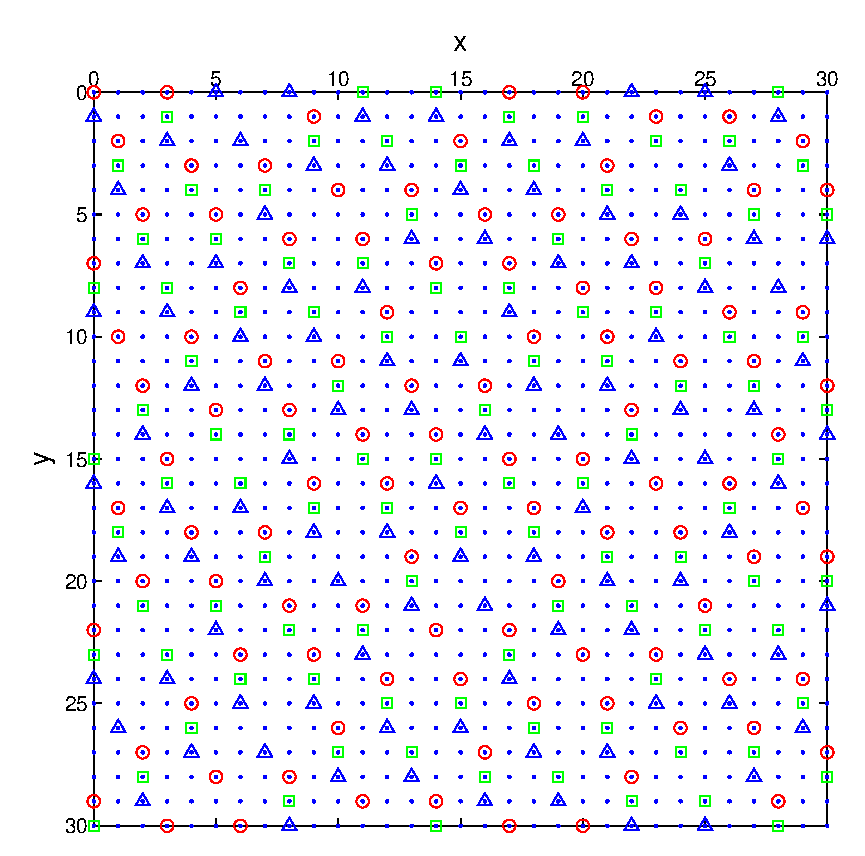
\includegraphics[width=7cm]{figure_sampling_view1.eps}
    \medskip
    \centerline{(a)}
  \end{minipage}\hfill
  \begin{minipage}[t]{0.49\linewidth}\centering
    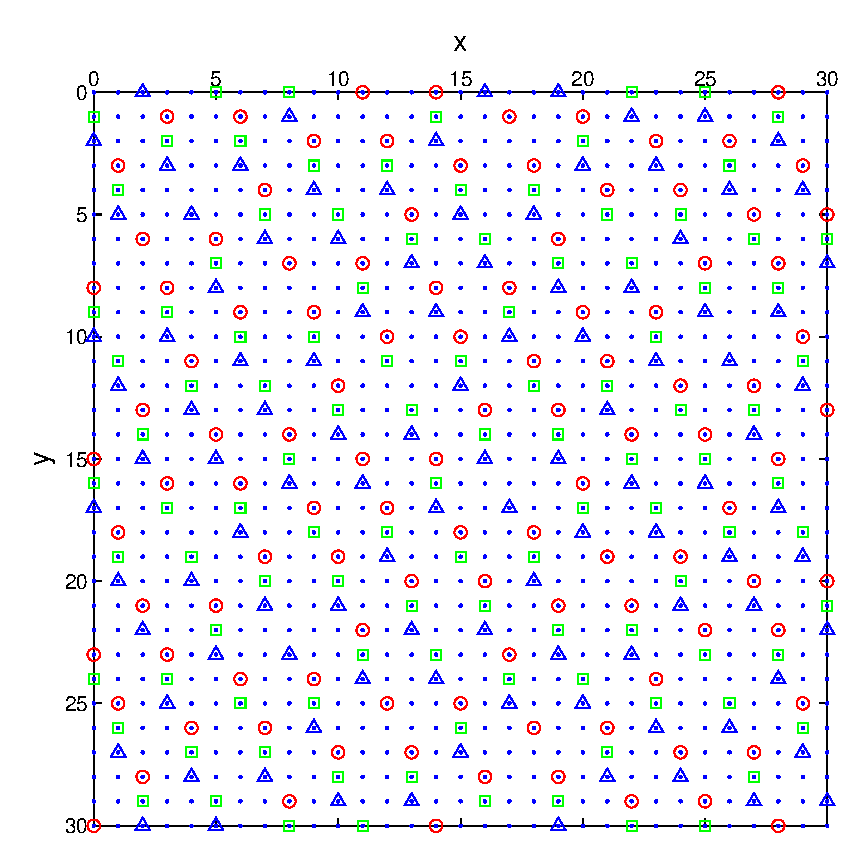
\includegraphics[width=7cm]{figure_sampling_view2.eps}
    \medskip
    \centerline{(b)}
  \end{minipage}
  \caption{Assignment of single-view intensities to RGB components: (a) view
    \#1; and (b) view \#2. }
  \label{fig:Sampling}
\end{figure}

You will also be using a lot of citations. Here is the format required in the dissertation: \cite{lamport1985:latex},\cite{Debr01}.

In all likelihood, you will need to insert tables. See one example on the next page.
\clearpage

\begin{table}[h]
	\caption{Absolute disparity error per pixel for the test data from
		Fig.~\ref{fig:Sampling} and different parameter values. In each experiment one
		parameter is adjusted while other parameters are unchanged.} 
	\centering
	\begin{minipage}[b]{0.30\linewidth}
		\centerline{$\eta=6000$, $\mu=2000$}\smallskip
		\centering
		\begin{tabular}{ccc}
			\hline
			$K$ & $u_1$ & $u_2$\\
			\hline
			3   & 0.52 &0.46\\
			7   & 0.47 &0.43\\
			10  & 0.35 &0.36\\
			12  & 0.37 &0.36\\
			\hline
		\end{tabular}
	\end{minipage}
	%
	\begin{minipage}[b]{0.34\linewidth}
		\centerline{$K=10$, $\mu=2000$}\smallskip
		\centering
		\begin{tabular}{ccc}
			\hline
			$\eta$ & $u_1$ & $u_2$\\
			\hline
			1000&0.54& 0.45\\
			3000&0.43& 0.40\\
			6000&0.35& 0.36\\
			9000&0.37& 0.37\\
			\hline
		\end{tabular}
	\end{minipage}
	%
	\begin{minipage}[b]{0.32\linewidth}
		\centerline{$K=10$, $\eta=6000$}\smallskip
		\centering
		\begin{tabular}{ccc}
			\hline
			$\mu$ & $u_1$ & $u_2$\\
			\hline
			100 &1.00&1.16\\
			1000&0.53&0.47\\
			2000&0.35&0.36\\
			3000&0.44&0.43\\
			\hline
		\end{tabular}
	\end{minipage}
	%
	\label{tab:Parameters}
\end{table}

\section{Experiment of Memory Allocation}
\label{sec:history}
This experiment is to test how static and dynamic memory allocation of Java and Rust behave. For the assessment, Element addition to ArrayList in the case of Java and Vector in the case of Rust 
is emploied here. These data stractures are resizable and we have control to set initial size. There are two parameters; initial size of ArrayList or Vector and thier final size after additions of elements. 
We are interested in the impact to memory allocation by initial allocation and expantion to runtime.

First, an ArrayList and an Vector are created with specified initial size. Then, in a loop, a element is added for each iteration until the size of the ArrayList or Vector get the specified final size. 
Each data structure has a different resizing strategy. When an ArrayList hits current limit of its size and expands the limit, it doubles the current size.  
While Vector does not have specific strategy for its resizing, the expantions of size of both ArrayList and Vector might affect the digradation of runtime performance.

To perform benchmarks, we use Java Microbenchamrk Hardness (JMH) for Java and Criterion for Rust. The benchmark time is calculated mean from several iterarions. 
We warm up before the execution. The parameters are set in combination of initial size, 10, 100, 1000, and 10000 and final size, 9, 99, 999, 9999. 
The results are shown in Figure 2-4 and 2-5. 

Discussions here are separated to two cases: when initial size is set bigger than final size and when final size is set bigger than initial size. 
For ArrayList in Java, it shows performance significant degradation when the initial size is bigger than final size. When we create ArrayList with intial size of 1000 and add 99 elements 
to the ArrayList, the the average execution time is 1125 ns. However, the average excution time when we create ArrayList with intial size of 100 and add 99 elements is 623 ns. 
This degration is caused by the cost of initializing the large array. On the other hand, Rust Vector does not have significant cost for the initialization of size compared to the cost of addition of elements. 
In the case of Vector with initial size of 1000 and add 99 elements to the Vector, the average excution is 320 ns. In the case of the initial size of 100 and 99 elements additions, 
the average excution is 279 ns. This is such small degradation compared to element addition in Vector. 

In ArrayList when the initial size is smaller than the final size, there can be degradation in performance. When its initial size and final size are set 100 and 999 respectively, 
the average execution time is 10884 ns. However when its initial size and final size are set 1000 and 999 respectively, the average execution time is 4250 ns. 
This result shows the degradation of in performance caused by the copy of existing elements into newly allocated array whose size is double of the last array.

This characteristic can be seen in the case of Vector in Rust. Vector with initial size 100 and final size 999 performs the average excution time 3514 ns, 
but one with initial size 1000 and final size 999 performs 2723 ns. When the Vector reachs its capacity, it allocates a larger buffer and copies the present elements to it.
This cost results in the degradation of the average excution time.

\begin{figure}[htb]
    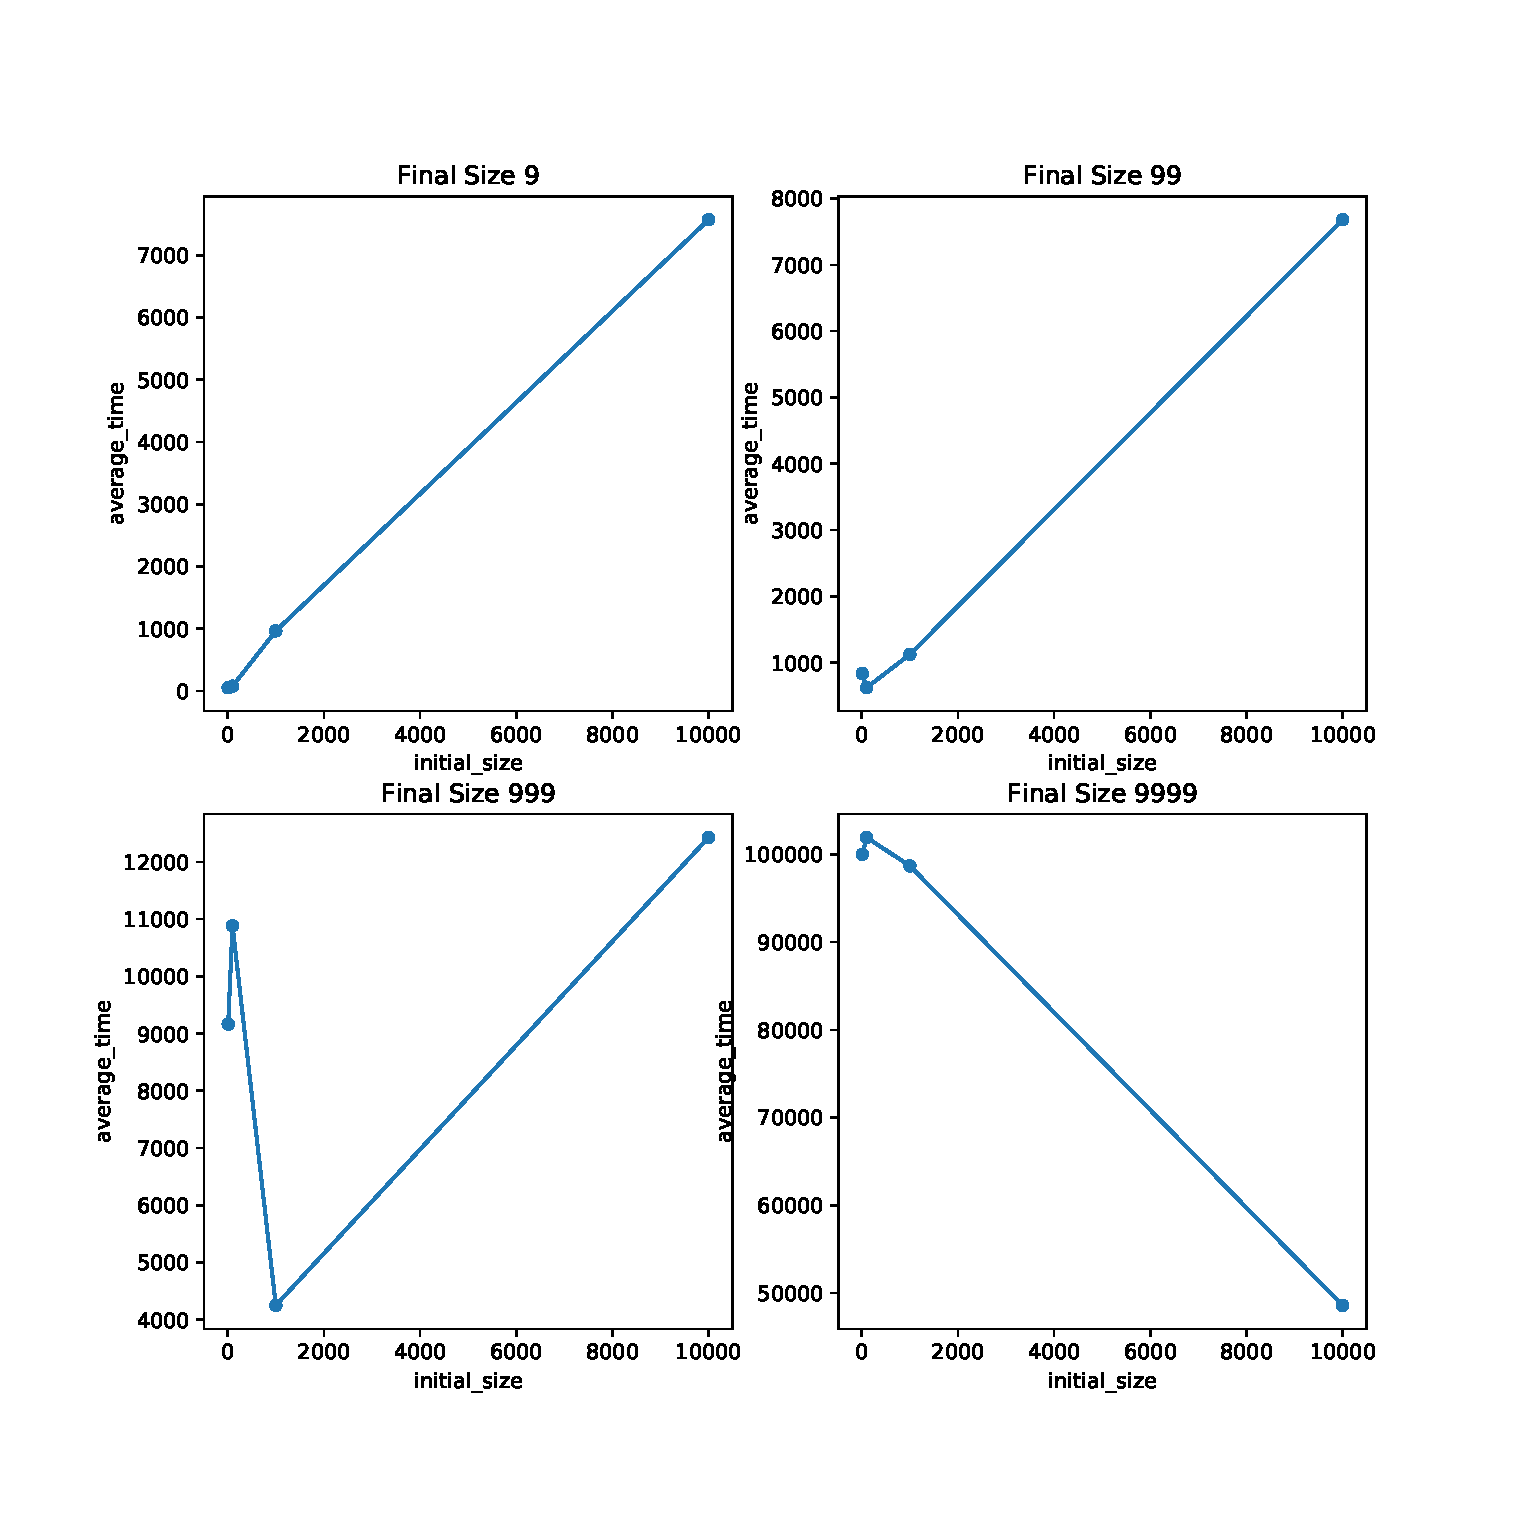
\includegraphics[width=15cm]{java_arraylist.eps}
    \caption{Memory allocation of ArrayList in Java}
    \label{fig:Sampling}
\end{figure}

\begin{figure}[htb]
    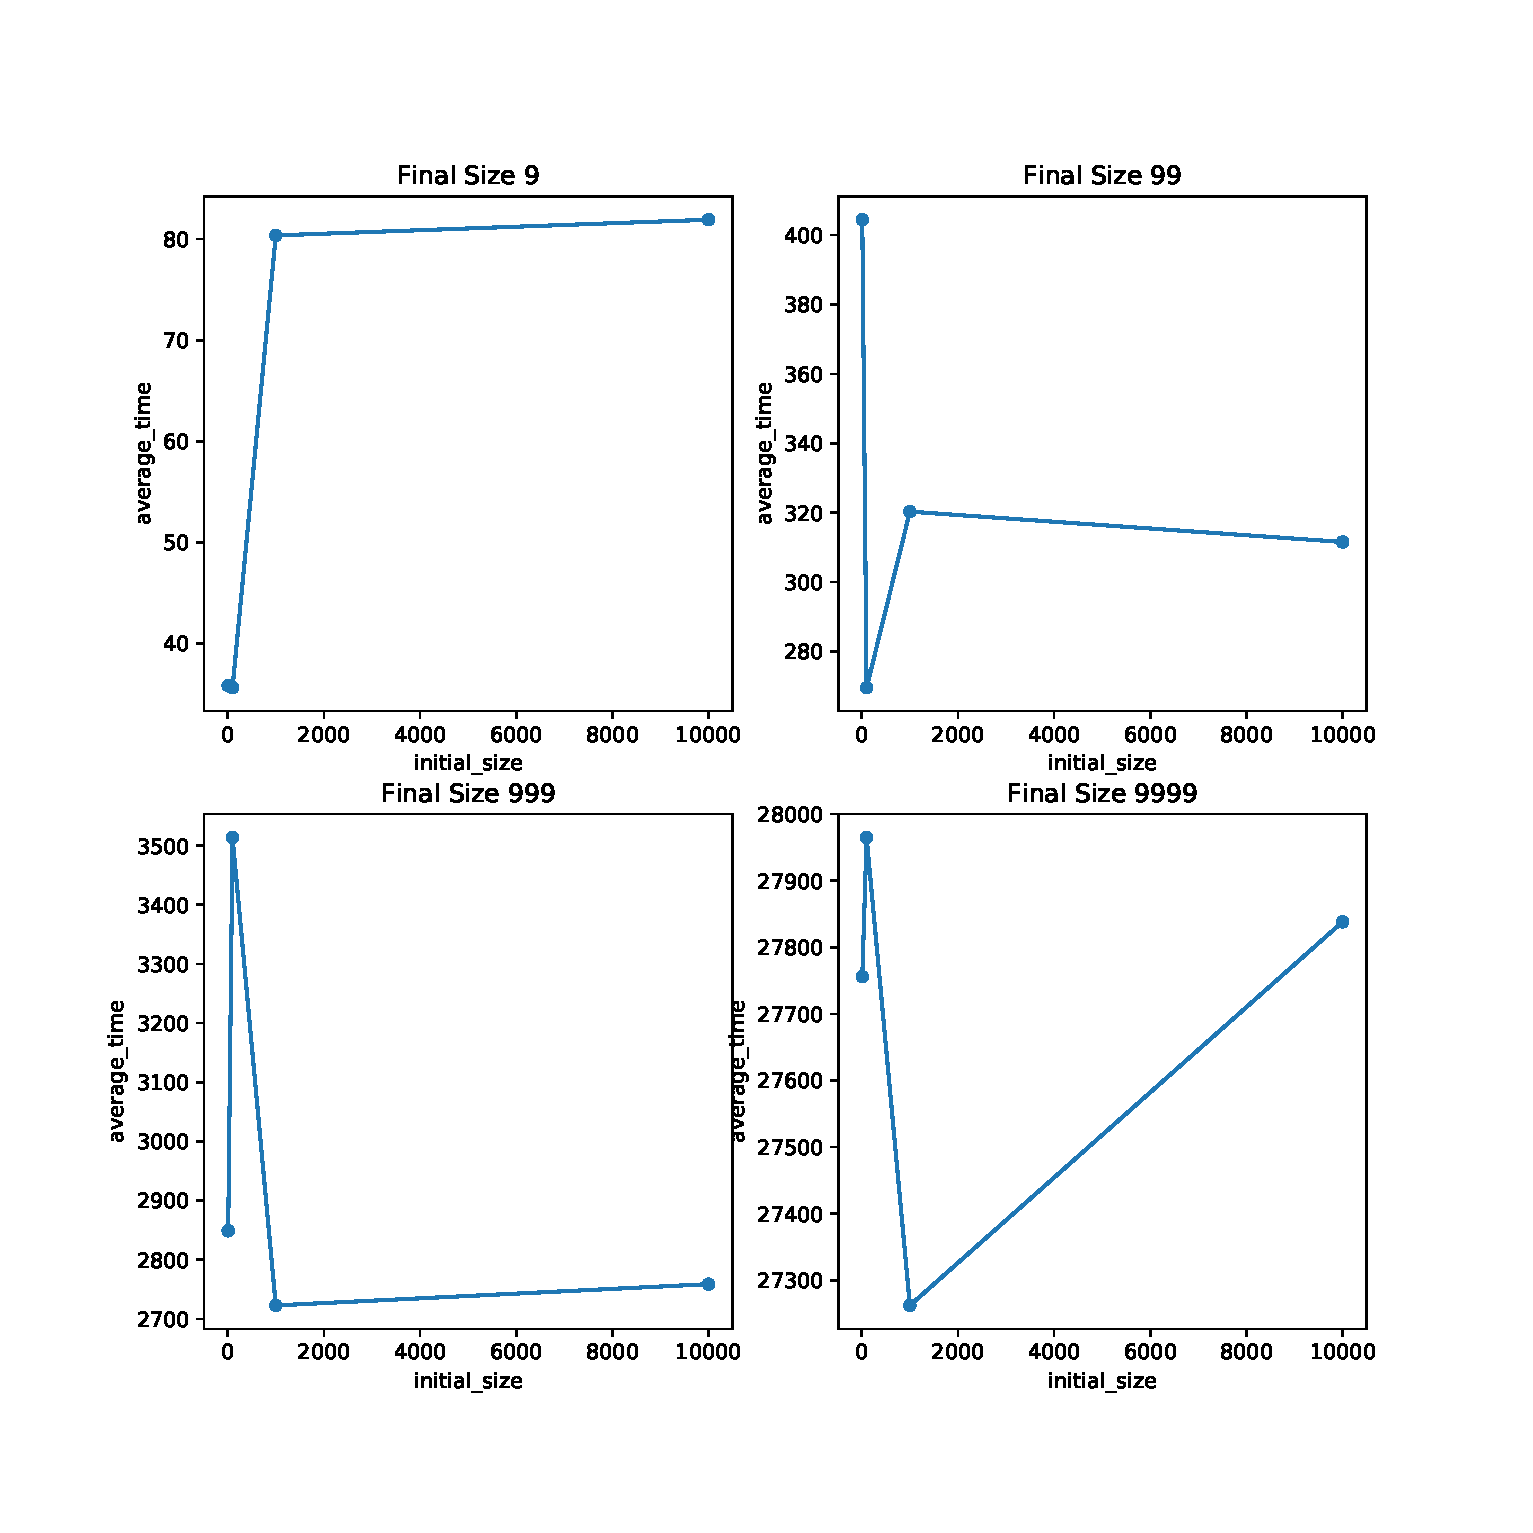
\includegraphics[width=15cm]{rust_vector.eps}
    \caption{Memory allocation of Vector in Rust}
    \label{fig:Sampling}
\end{figure}


\clearpage

\section{Experiment of Memory Allocation for Different Element Type.}
\label{sec:history}
This experiment is to test how static and dynamic memory allocation of Java and Rust behave. For the assessment, Element addition to ArrayList in the case of Java and Vector in the case of Rust 
is emploied here. These data stractures are resizable and we have control to set initial size. There are two parameters; initial size of ArrayList or Vector and thier final size after additions of elements. 
We are interested in the impact to runtime performance by initializing memory allocation and dynamicaly allocating memory space.

First, an ArrayList and an Vector are created with specified initial size. Then, in a loop, a element is added for each iteration until the size of the ArrayList or Vector get the specified final size. 
Each data structure has a different resizing strategy. When an ArrayList hits current limit of its size and expands the limit, it doubles the current size.  
While Vector does not have specific strategy for its resizing, the expantions of size of both ArrayList and Vector might affect the digradation of runtime performance.

Second, four types of element are used for elements addition to each data structure: integer, array of charactors, string, and Customer object. 
Assamption is that there would be different behavior between element additions of dynamically resizable and static size objects. 
Customer object has three fields. These fields are total order, weight of order, and zip code whose types are integer (i32 in rust), double (f32 in rust), and string respectively.
Figure 2-6 and 2-7 are representations of customer objects in Java and Rust.

Figure 2-10, 2-11, 2-12, and 2-13 represent the result of the experiments. For both data structures, integer elements addition shows the fastest runtime among all object types. 
This is because the compilers know each integer need 4 bytes to be stored in memory so that the space for memory that should be allocated is easily inspected. 
For the same reason, the initialization of data structures whose elements are integers alaways improves runtim performance.

The elements addition of strings and array of character behave similally among each languages. These two types of elements addition perform the similar speed and significantly slower than integer addition. 
Customer object addition is the slowest in Java. However, in Rust the addition of Customer object is the second fastest among all element typs.
The impacts of initialization of Java ArrayList vary among elemet types. On the other hand, the initailization Rust Vector always improves runtime performance for any of 4 types of elements addition.


\begin{figure}[htb]
    \begin{lstlisting}
        class Customer {
            int totalOrder;
            double weightOrder;
            String zipCode;
        }
    \end{lstlisting}
    \caption{Representation of Customer object in Java.}
    \label{fig:Sampling}    
\end{figure}

\begin{figure}[htb]
    \begin{lstlisting}
        struct Customer {
            total_order: i32,
            weight_order: f32,
            zip_code: String,
        }
    \end{lstlisting}
    \caption{Representation of Customer object in Rust.}
    \label{fig:Sampling}
\end{figure}

\begin{figure}[htb]
    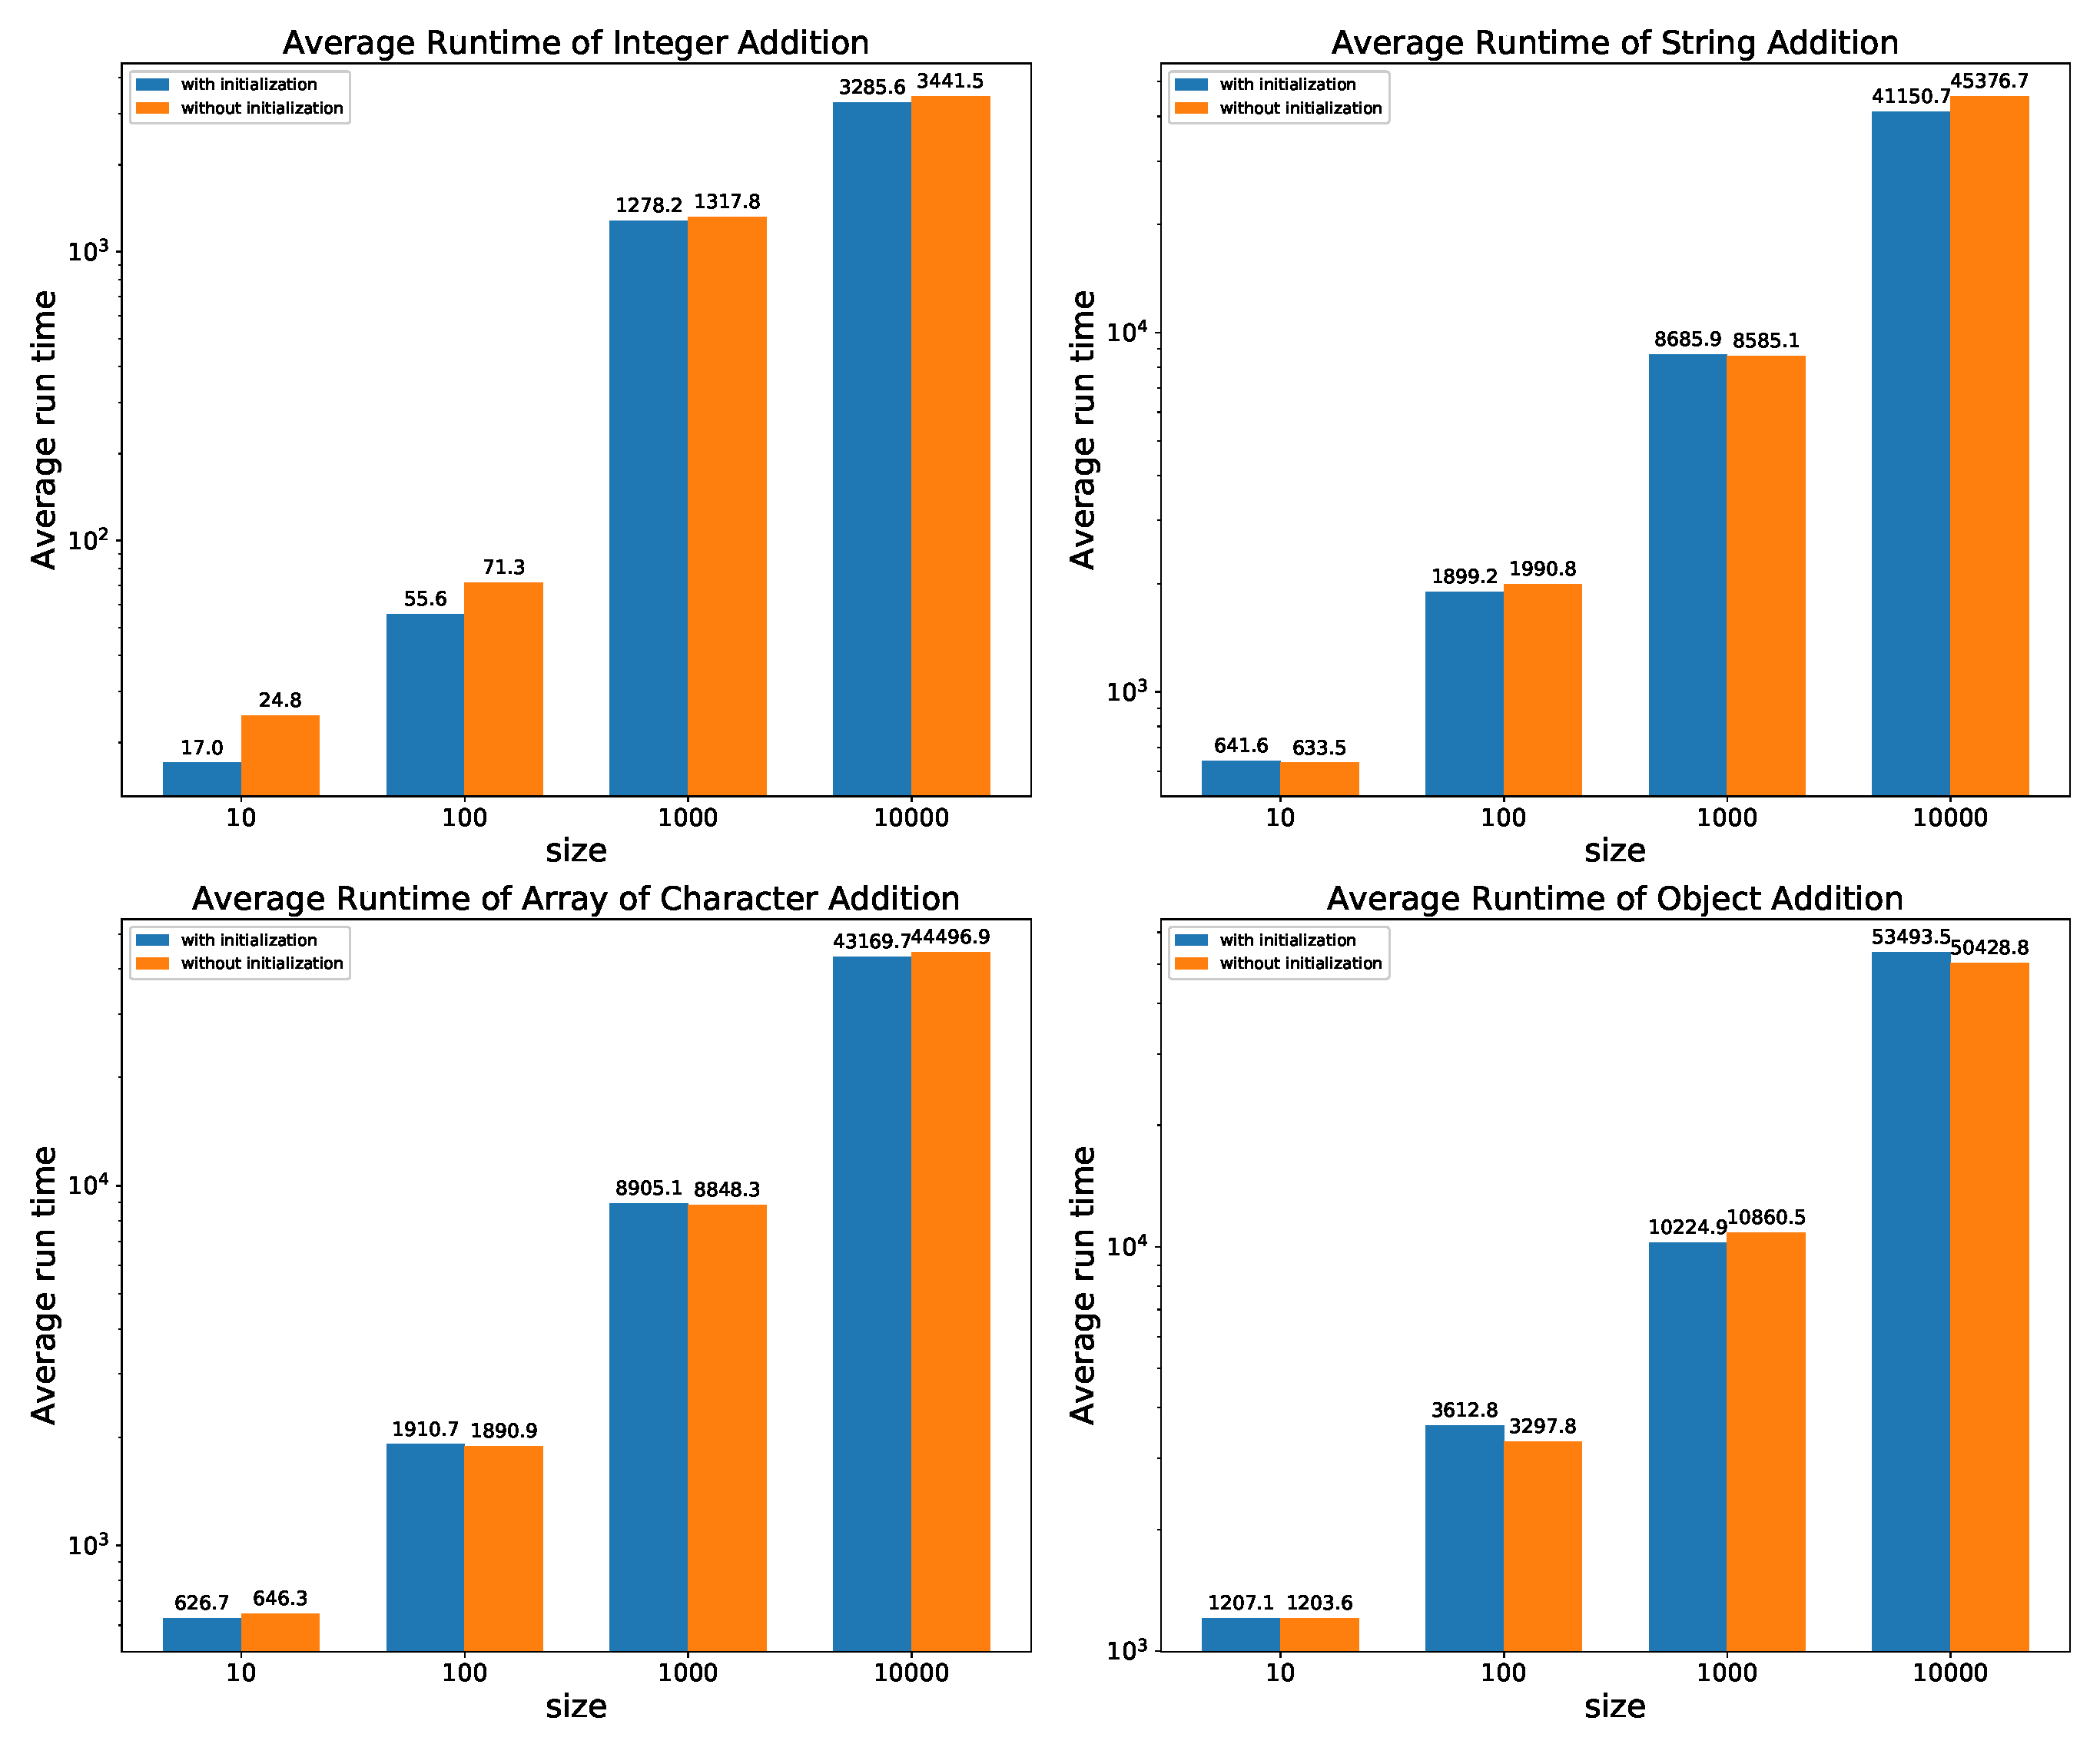
\includegraphics[width=15cm]{java_arraylist_log.eps}
    \caption{Memory allocation of Java ArrayList}
    \label{fig:Sampling}
\end{figure}

\begin{figure}[htb]
    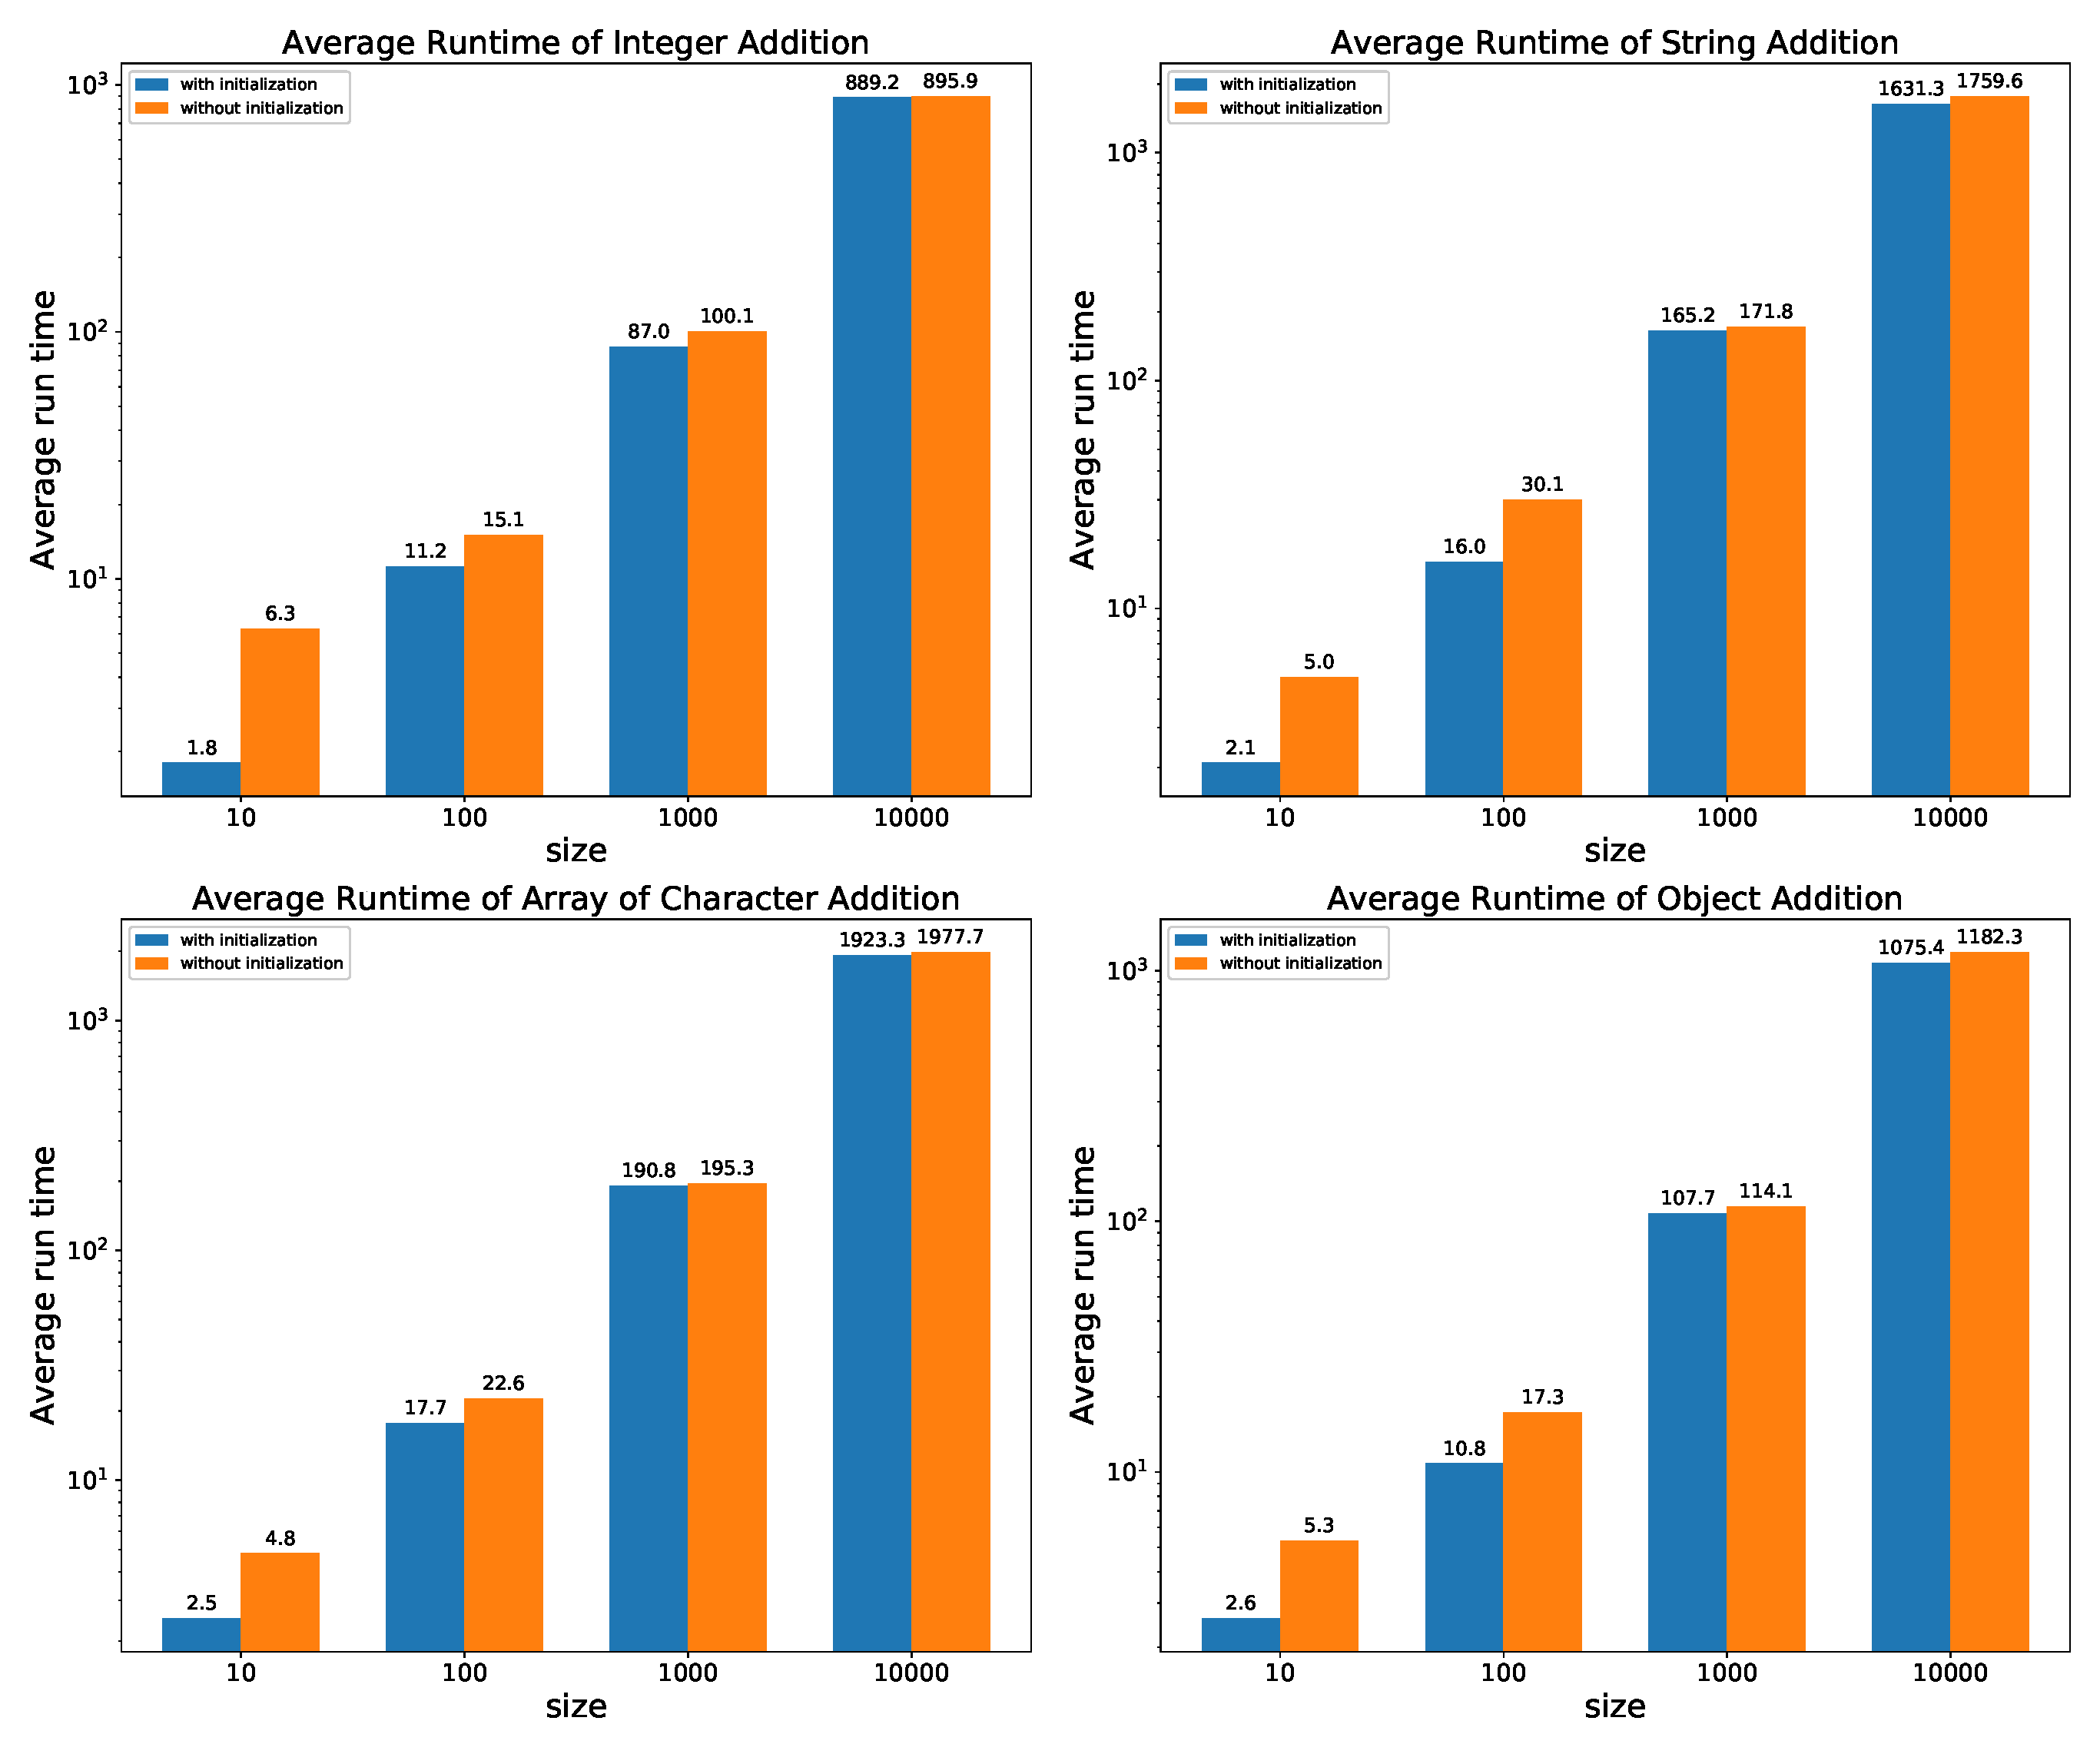
\includegraphics[width=15cm]{rust_vector_log.eps}
    \caption{Memory allocation of Rust Vector}
    \label{fig:Sampling}
\end{figure}


\begin{figure}[htb]
    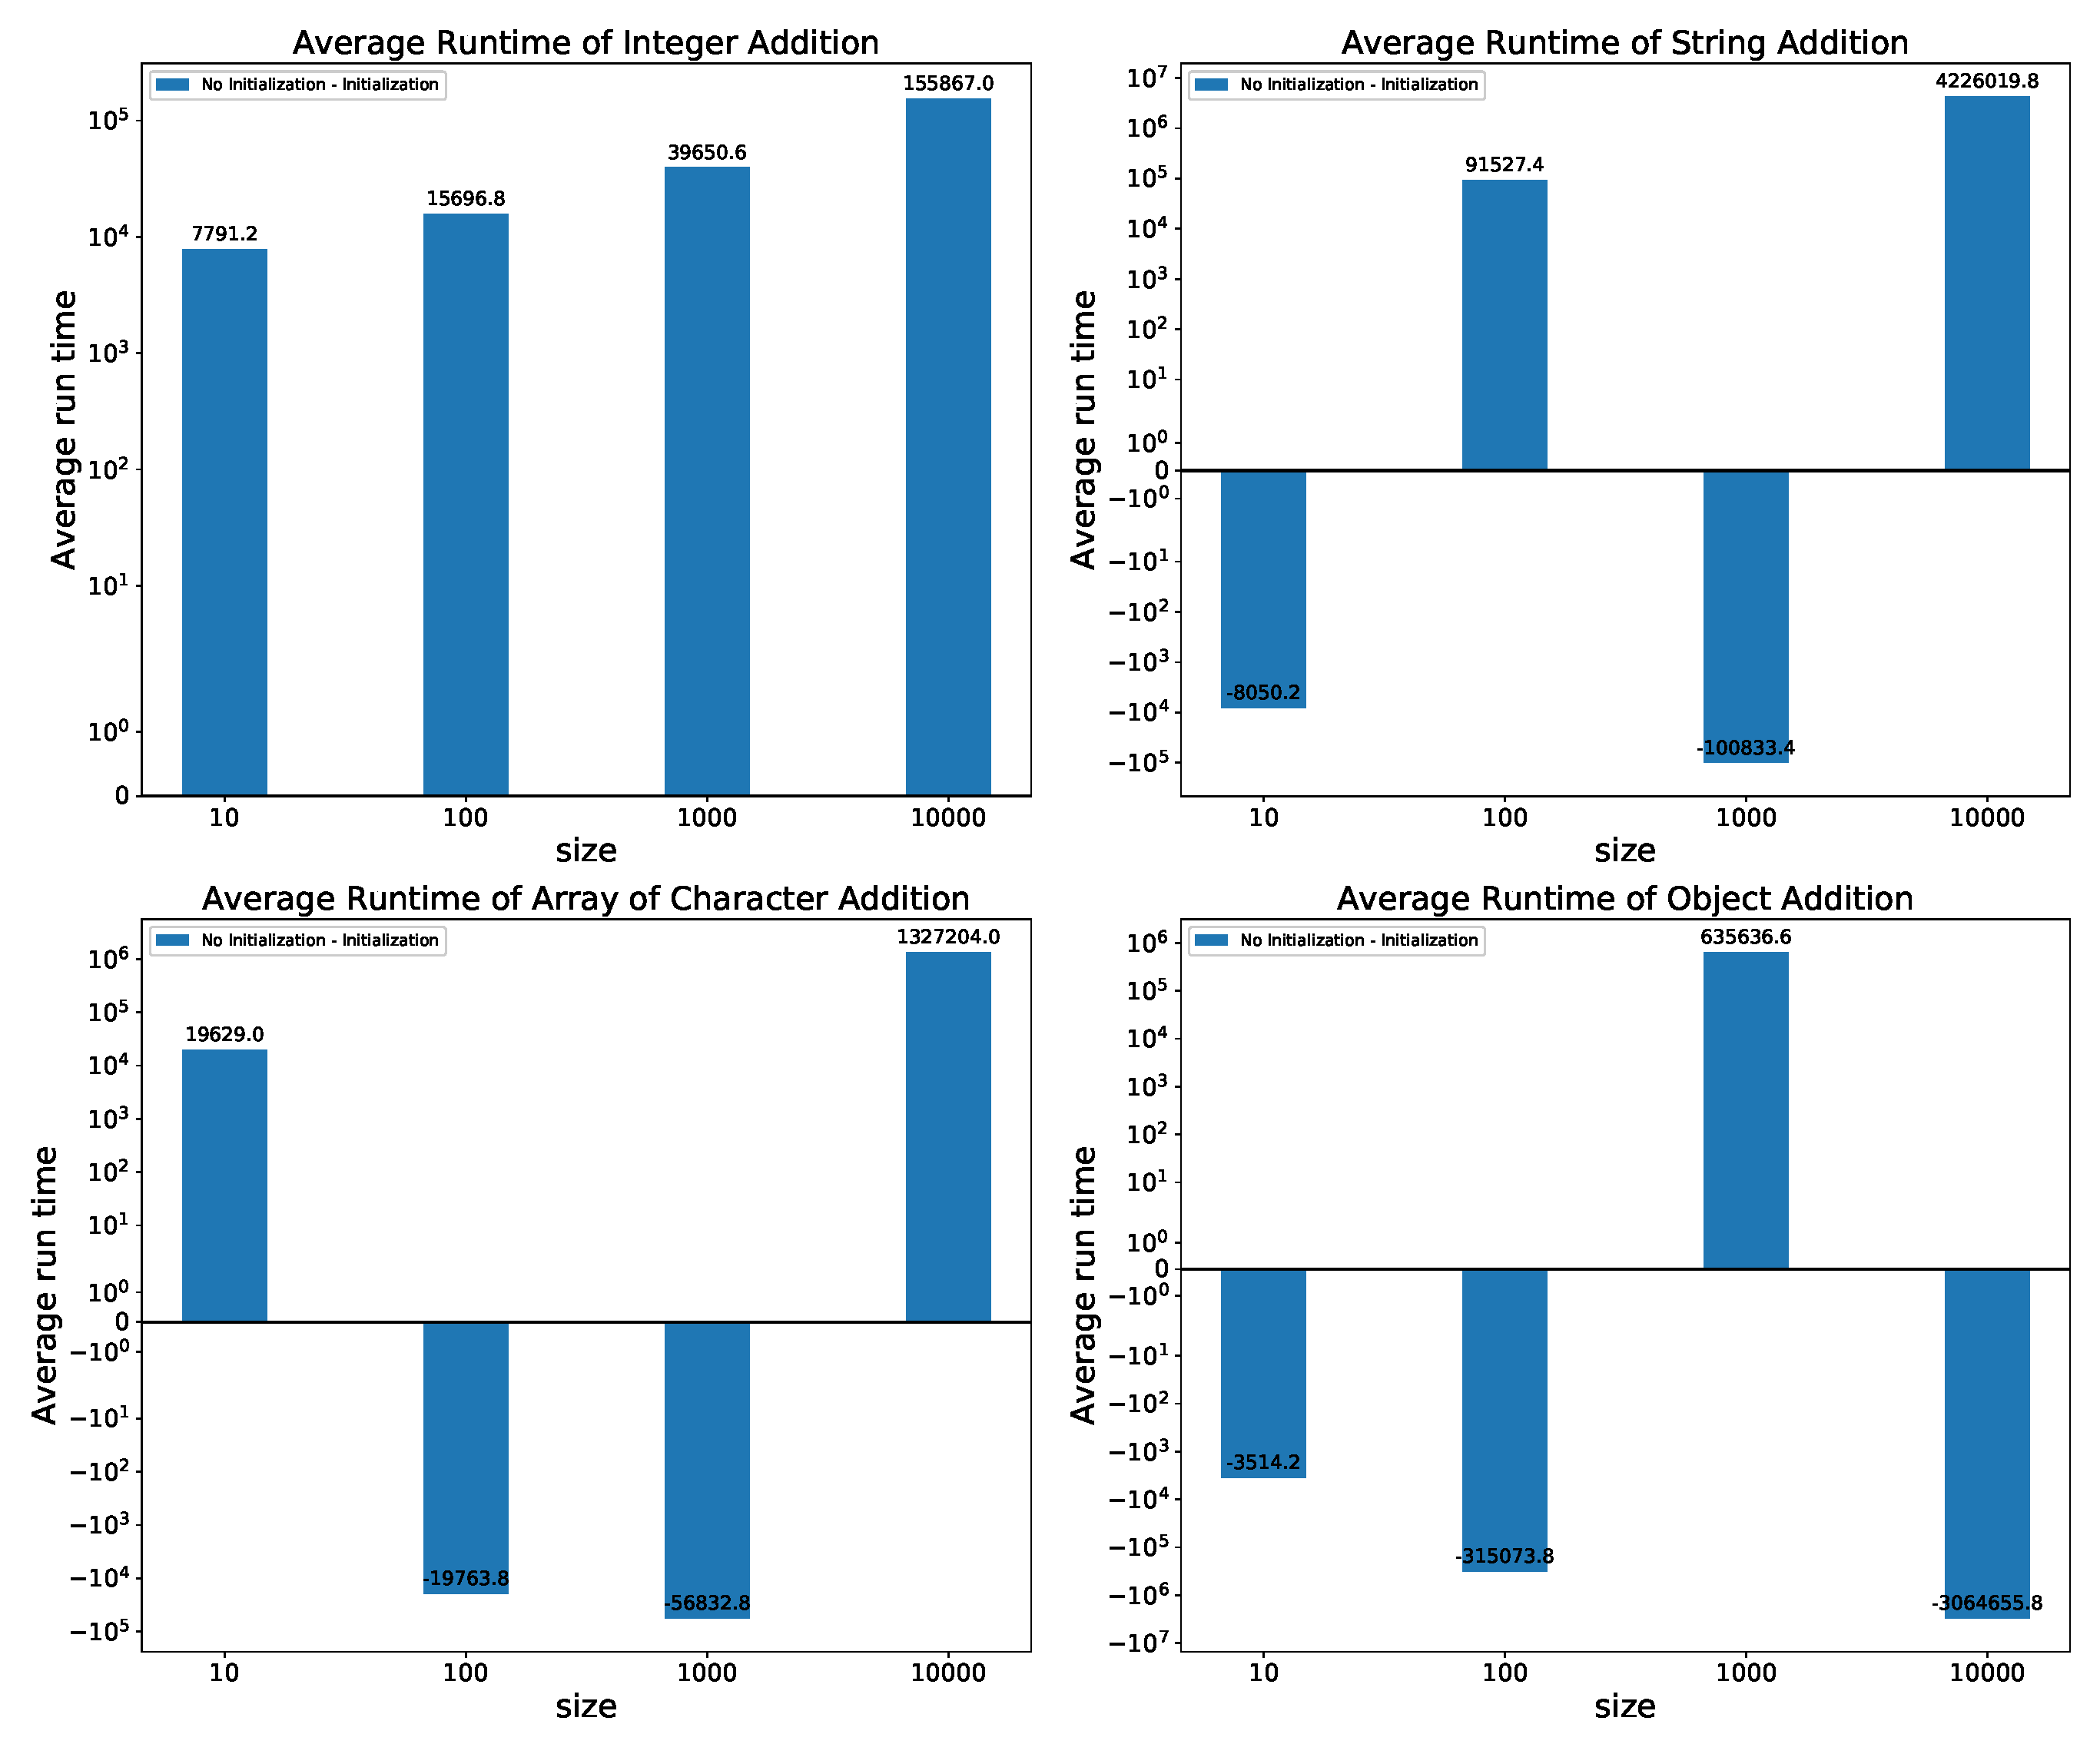
\includegraphics[width=15cm]{java_arraylist_difference.eps}
    \caption{Difference of Memory allocation of Java ArrayList between Non-initialization and Initialization}
    \label{fig:Sampling}
\end{figure}

\begin{figure}[htb]
    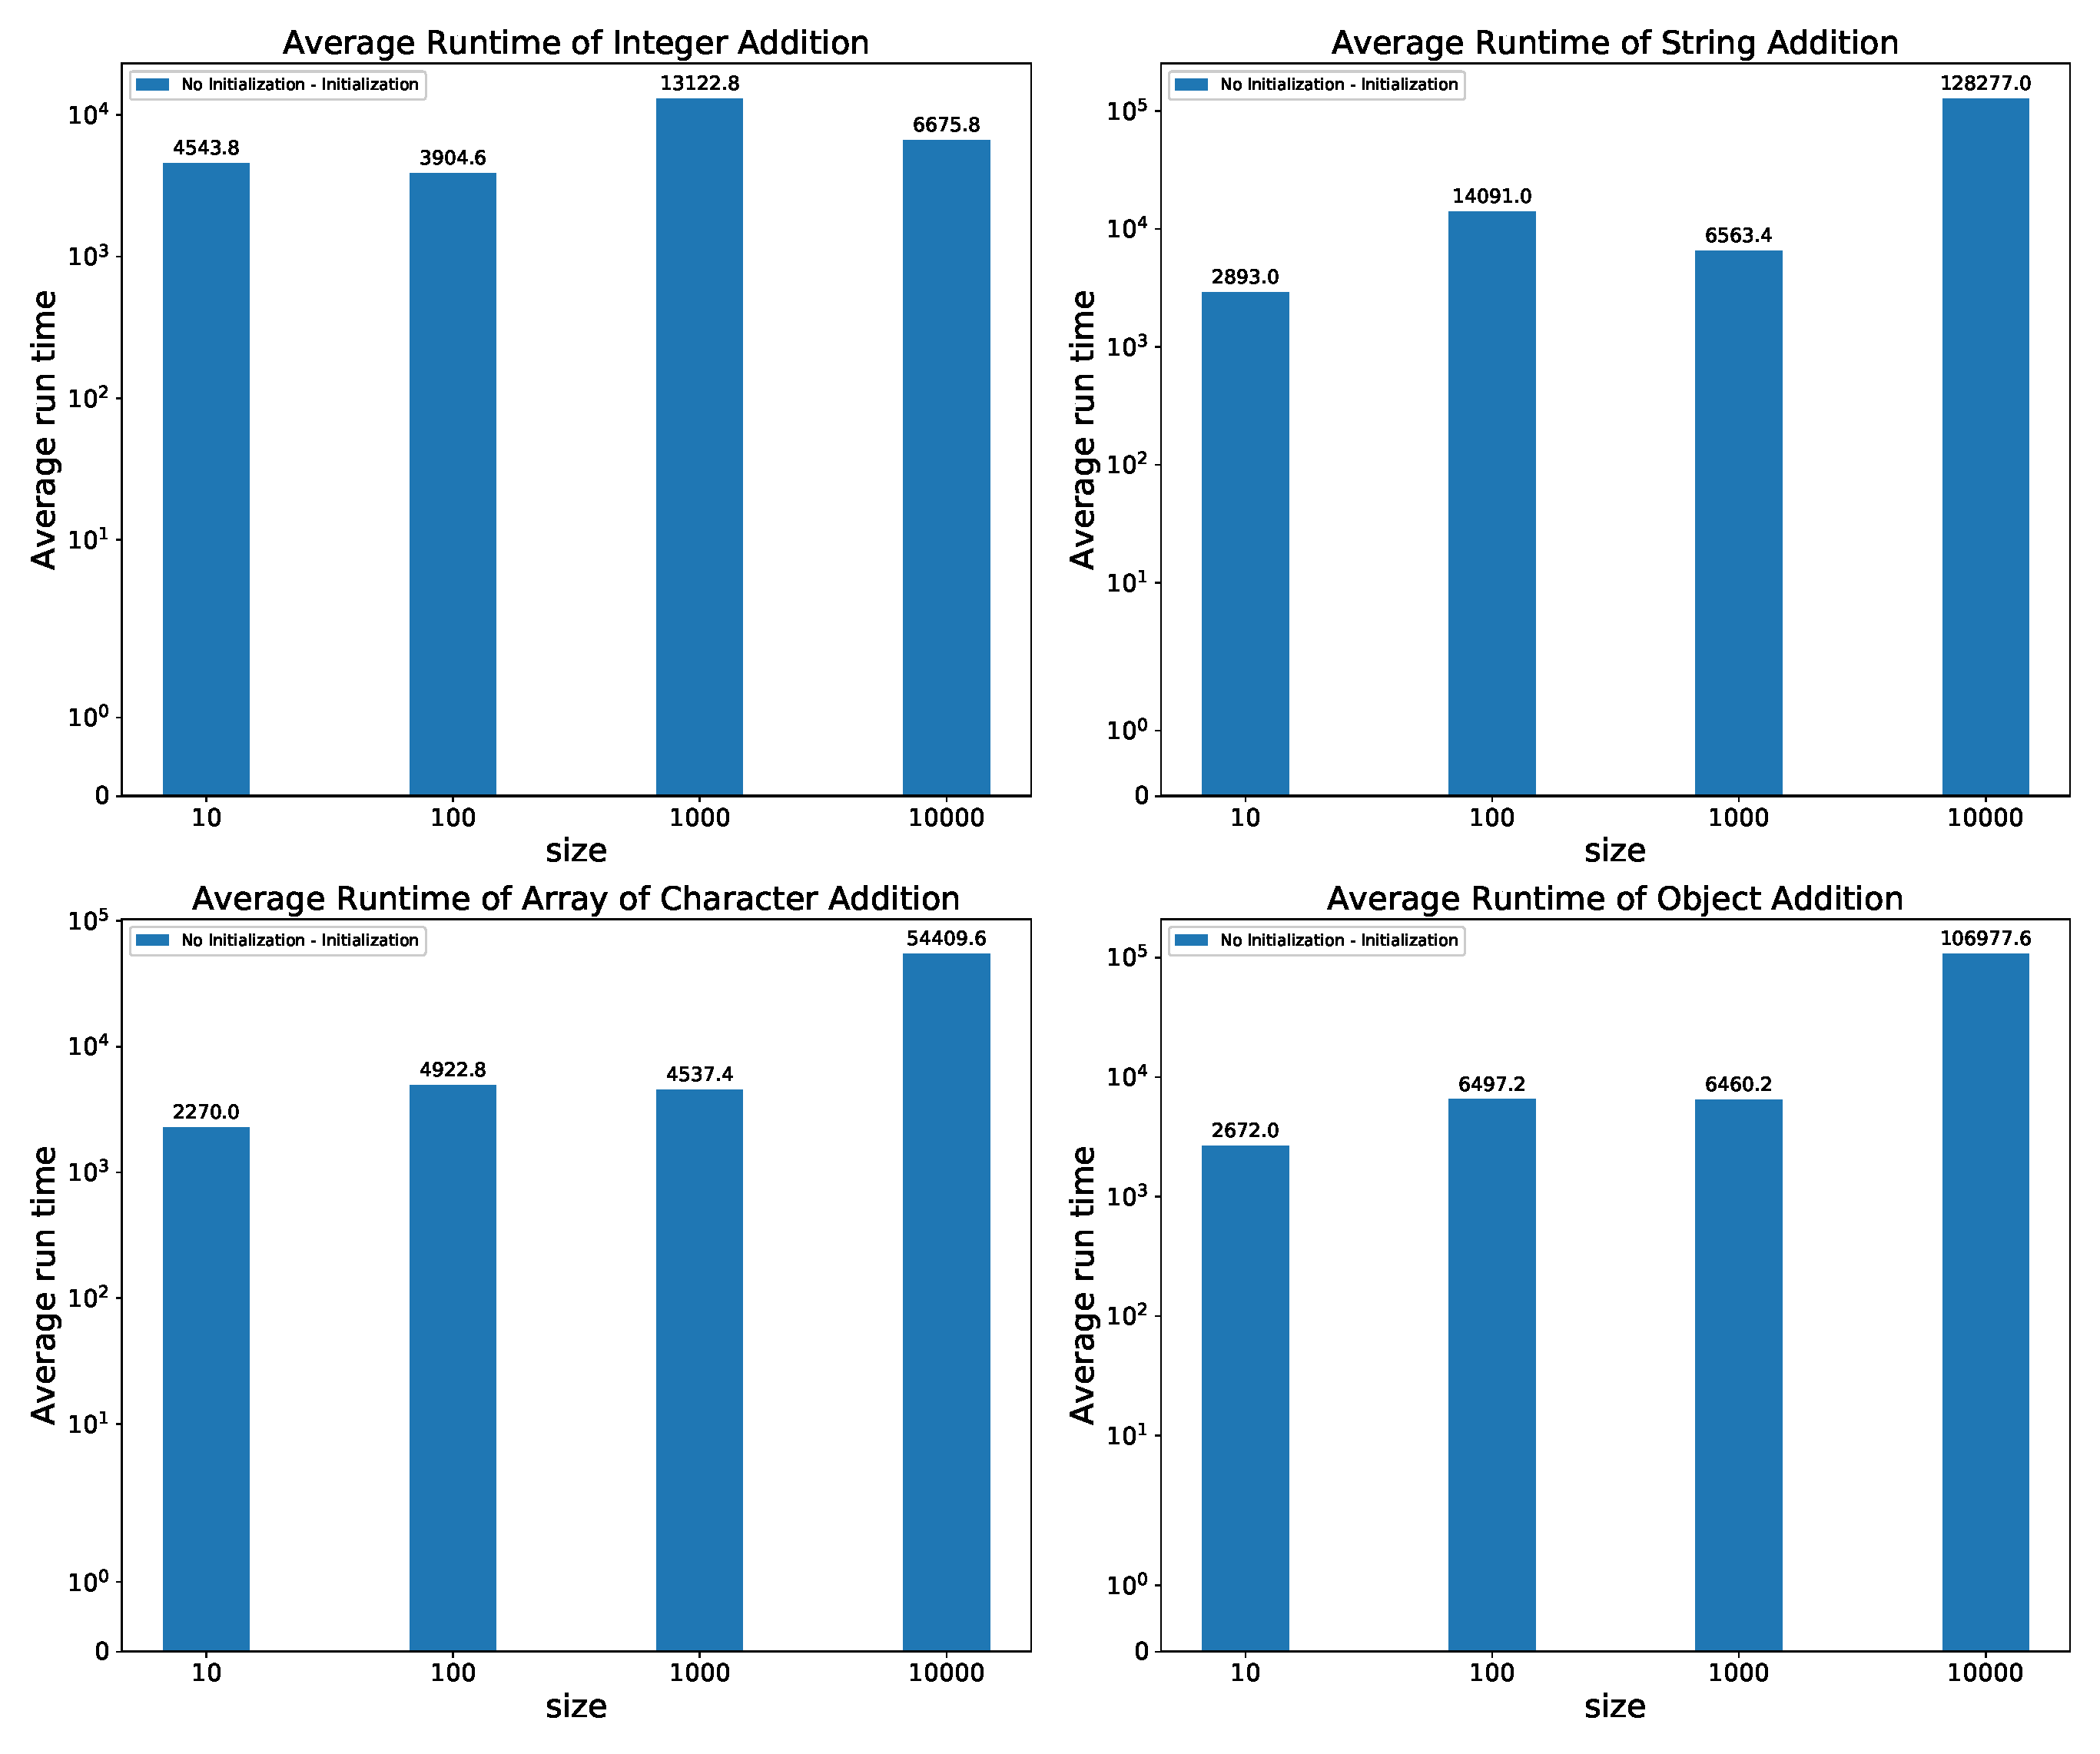
\includegraphics[width=15cm]{rust_arraylist_difference.eps}
    \caption{Difference of Memory allocation of Rust Vector between Non-initialization and Initialization}
    \label{fig:Sampling}
\end{figure}
\clearpage

\section{Assessment of different reference methods in Rust}
\label{sec:history}
% In Rust programming, a reference is a pointer to reduce unnecessary movement of ownership. 
% One use case is where we pass reference to values to arguments of function. 
% If we pass owner to function, the owner is moved and the corresponding value is deallocated when the call of function ends. 
% To avoid this, the owner should always be returned. This may be an encumbrance while complex software system development. 
% By using reference, we do not have to worry about returning it, because reference is an additional pointer to an owned value. 
% Reference can be used for operation in the same way of owner, but also be moved without deallocation of value by keeping its owner live. 

% Reference is useful to avoid movement of ownership. However, one needs to track its lifetime and explicitly includes it in code, 
% because Rust compiler cannot infer it. This can be another encumbrance. We can instead acquire multiple owners to single value by using Reference Counting (Rc). 
% By leveraging Rc, a value can be shared like what borrowing plays the role in Rust programming. 
% The difference is that Rc checks number of owner pointing to the actual data and makes sure the data is not deleted 
% until all the owners are dereferenced. Using Rc is sometimes preferable approach for developers especially when lifetime planning is extremely difficult.
% However, the possible problem regarding to Rc is the cost for tracking the number of references. 
% Having this assumption, this experiment will show difference of behavior among Rc and simple reference.

In this experiment, CustomerBorrowed and CustomerRc are used to see difference of dropping time among reference and Rc. 
In the CustomerRc and OrderRc struct, all fields take Rc (Rc$<$T$>$). Similarly to the experiment in the last section, 
sets of integer, float, and String vector are created and their elements are borrowed or reference counted to create CustomerBorrowed or CustomerRc objects.
The dropping of objects deletes references or Rcs used for fields of the objects. However, it does not deallocate values to which they are pointing. 
Therefore, the evaluated runtime of dropping objects only consists of dropping time of reference or Rc, but deallocation time.
We generated 10, 20, 30, and 40 million CustomerBorrowed and CustomerRc objects and performed drop one by one. 

\subsection{Result}
Figure\ref{fig:rc_ref} shows comparison of runtime dropping CustomerBorrowed and CustomerRc objects. 
The result shows significant difference of dropping time among the two objects; deletion of CustomerRc is much slower than CustomerBorrowed. 
The runtime of dropping CustomerBorrowed is about 60 times faster than dropping CustomerRc. 
The memory usage for algorithms with 40 million of Customer objects are about 26G bytes for both CustomerRc and CustomerBorrowed.

\begin{figure}[htb!]
    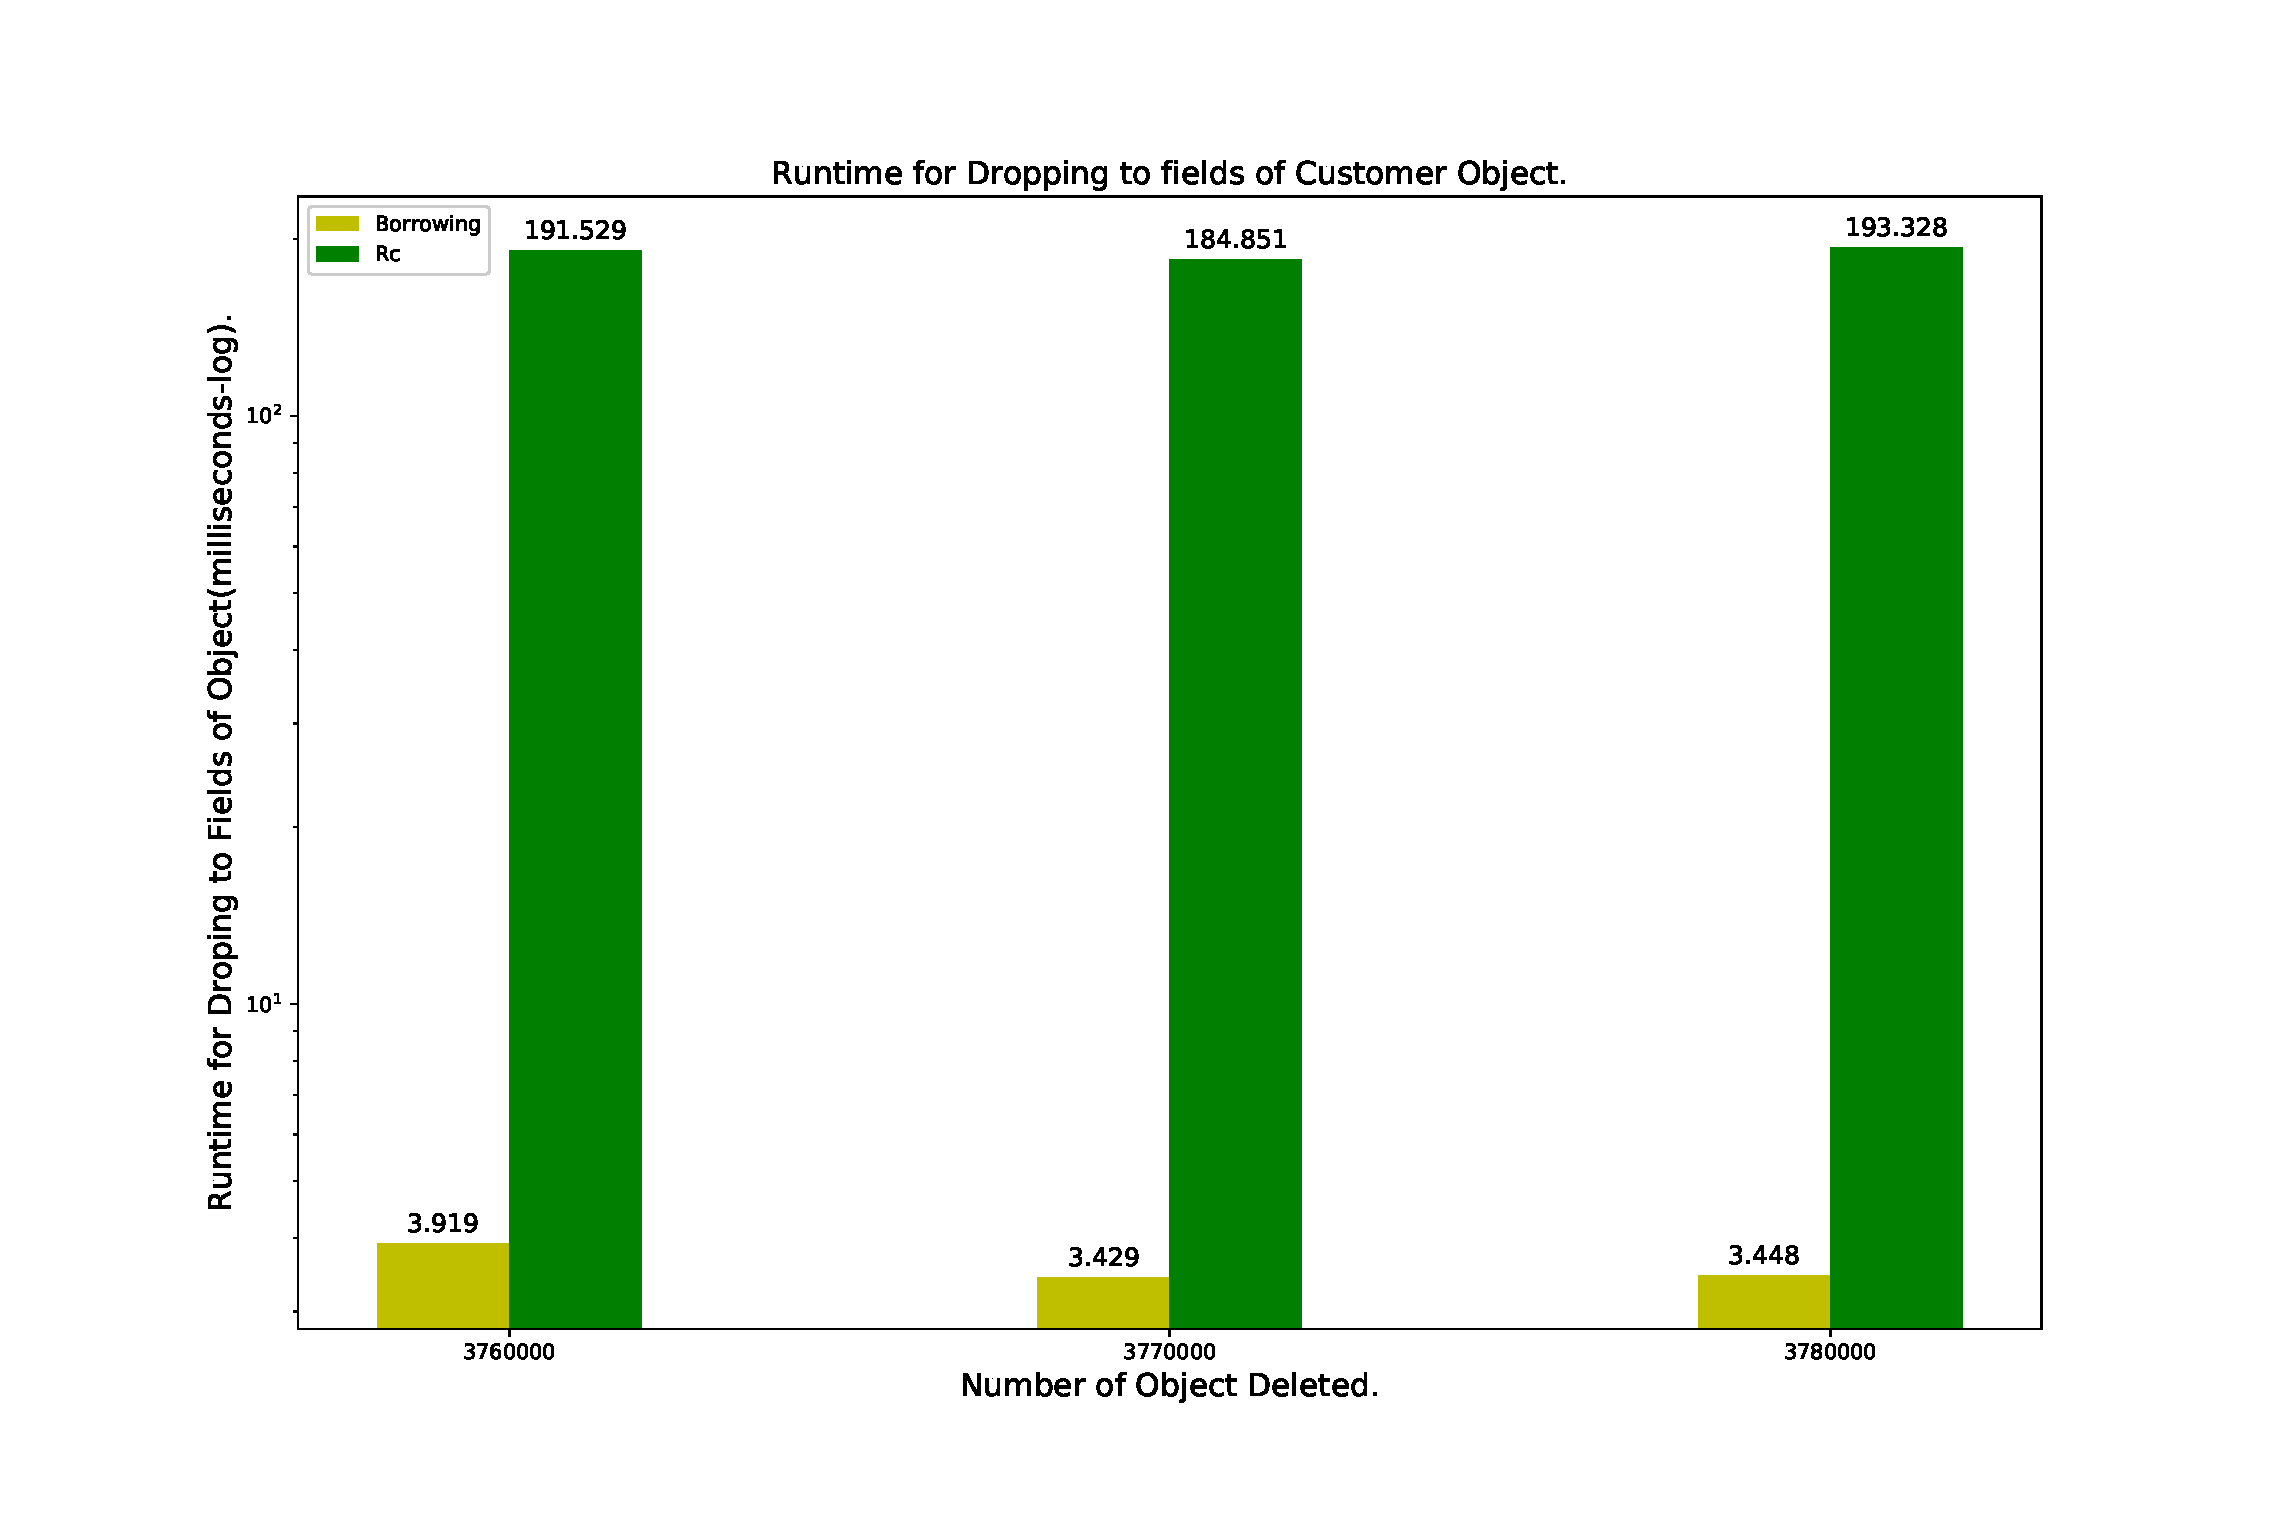
\includegraphics[width=15cm]{rust_droptime_borring_rc.eps}
    \caption{Runtime for dropping Customer Object}
    \label{fig:rc_ref}
\end{figure}


\subsection{Discussion}
In this experiment, an assessment is conducted to verify whether there is difference between behavior of reference and Rc.
The reason why dropping Rc is much slower than dropping reference is that Rc requires runtime overhead to check some states of the variable, 
but when to drop reference is already determined at compile time. When dropping Rc, Rc has to check the number of variables pointing to the actual content and decide 
whether to deallocate the memory or not. However, memory management and lifetime strategy of reference is already determined at compile time.
This determination of memory management strategy at compile increases runtime performance of dropping complex object constructed with reference type variable.
This may say that we should use reference whenever high performance computation is critical.

However, dealing with reference is sometimes cumbersome. Tracking lifetime of reference can be done easily in simple situation. 
But, if we have complex objects constructed with fields of reference, the lifetime tracking becomes extremely difficult. 
For example, constructing nested objects with reference fields requires a developer to plan memory management with many lifetime symbols. 
Using reference counting eliminates the developer's responsibility to specify lifetime of variables. 
This may ease and speed up development process, and increase understandability of codes.

Even though we have stack allocated values, such as i32 and f64, in Rc in our experiment, 
one should avoid wrapping stack allocated values in Rc. Wrapping value in Rc allocates heap memory so that allocating Rc$<$i32$>$ or Rc$<$f64$>$ unnecessarily uses space of 
heap. Additionally, stack allocated values are usually easy to be copied. Therefore, developer does not have to even use reference; one can just copy the value. 
Copying value in Rust is to copy the original value and to assign the copy to new owner variable. 
\clearpage

\section{Experiment for Merge-sort}
\label{sec:history}
This experiment is to assess importance of careful memory management in multithreading of Rust. 
We implement merge-sort algorithm in two different ways. One is sharing source vector with Arc. 
The other is passing slice of source vector to child thread. 

Our merge-sort algorithm with vector is implemented with recursion. In these alogorithm, the splitting phase is merely aquiring index of split position, 
not actually splitting the source vector. At merge phase, merge function receives two independent vector and merge these into single new vector.

For sharing data implementaion, channel with sending data is used for multithreading method, because we want to ensure children threads return values before parent thread proceed execution. 
For passing slice implementation, we use scope method to enable children threads to receive reference from their parent ensuring the same purpose of sending data. 

Experiment performed is the comparison among sharing data and passing slice implementations to see the impact of Arc, Atomic reference conuting, to runtime performance.
These two implementations are theoritically the same operations other than using or not using Arc to share data. 
This comparison can effectively show how important careful memory management is in multithreading computation in Rust. 
In another word, how atomic reference counting can cost for computation in Rust programming.

The figure shows the result of 
An atomic reference count of the shareable vector is passed to every recursion steps and 


\begin{figure}[htb]
    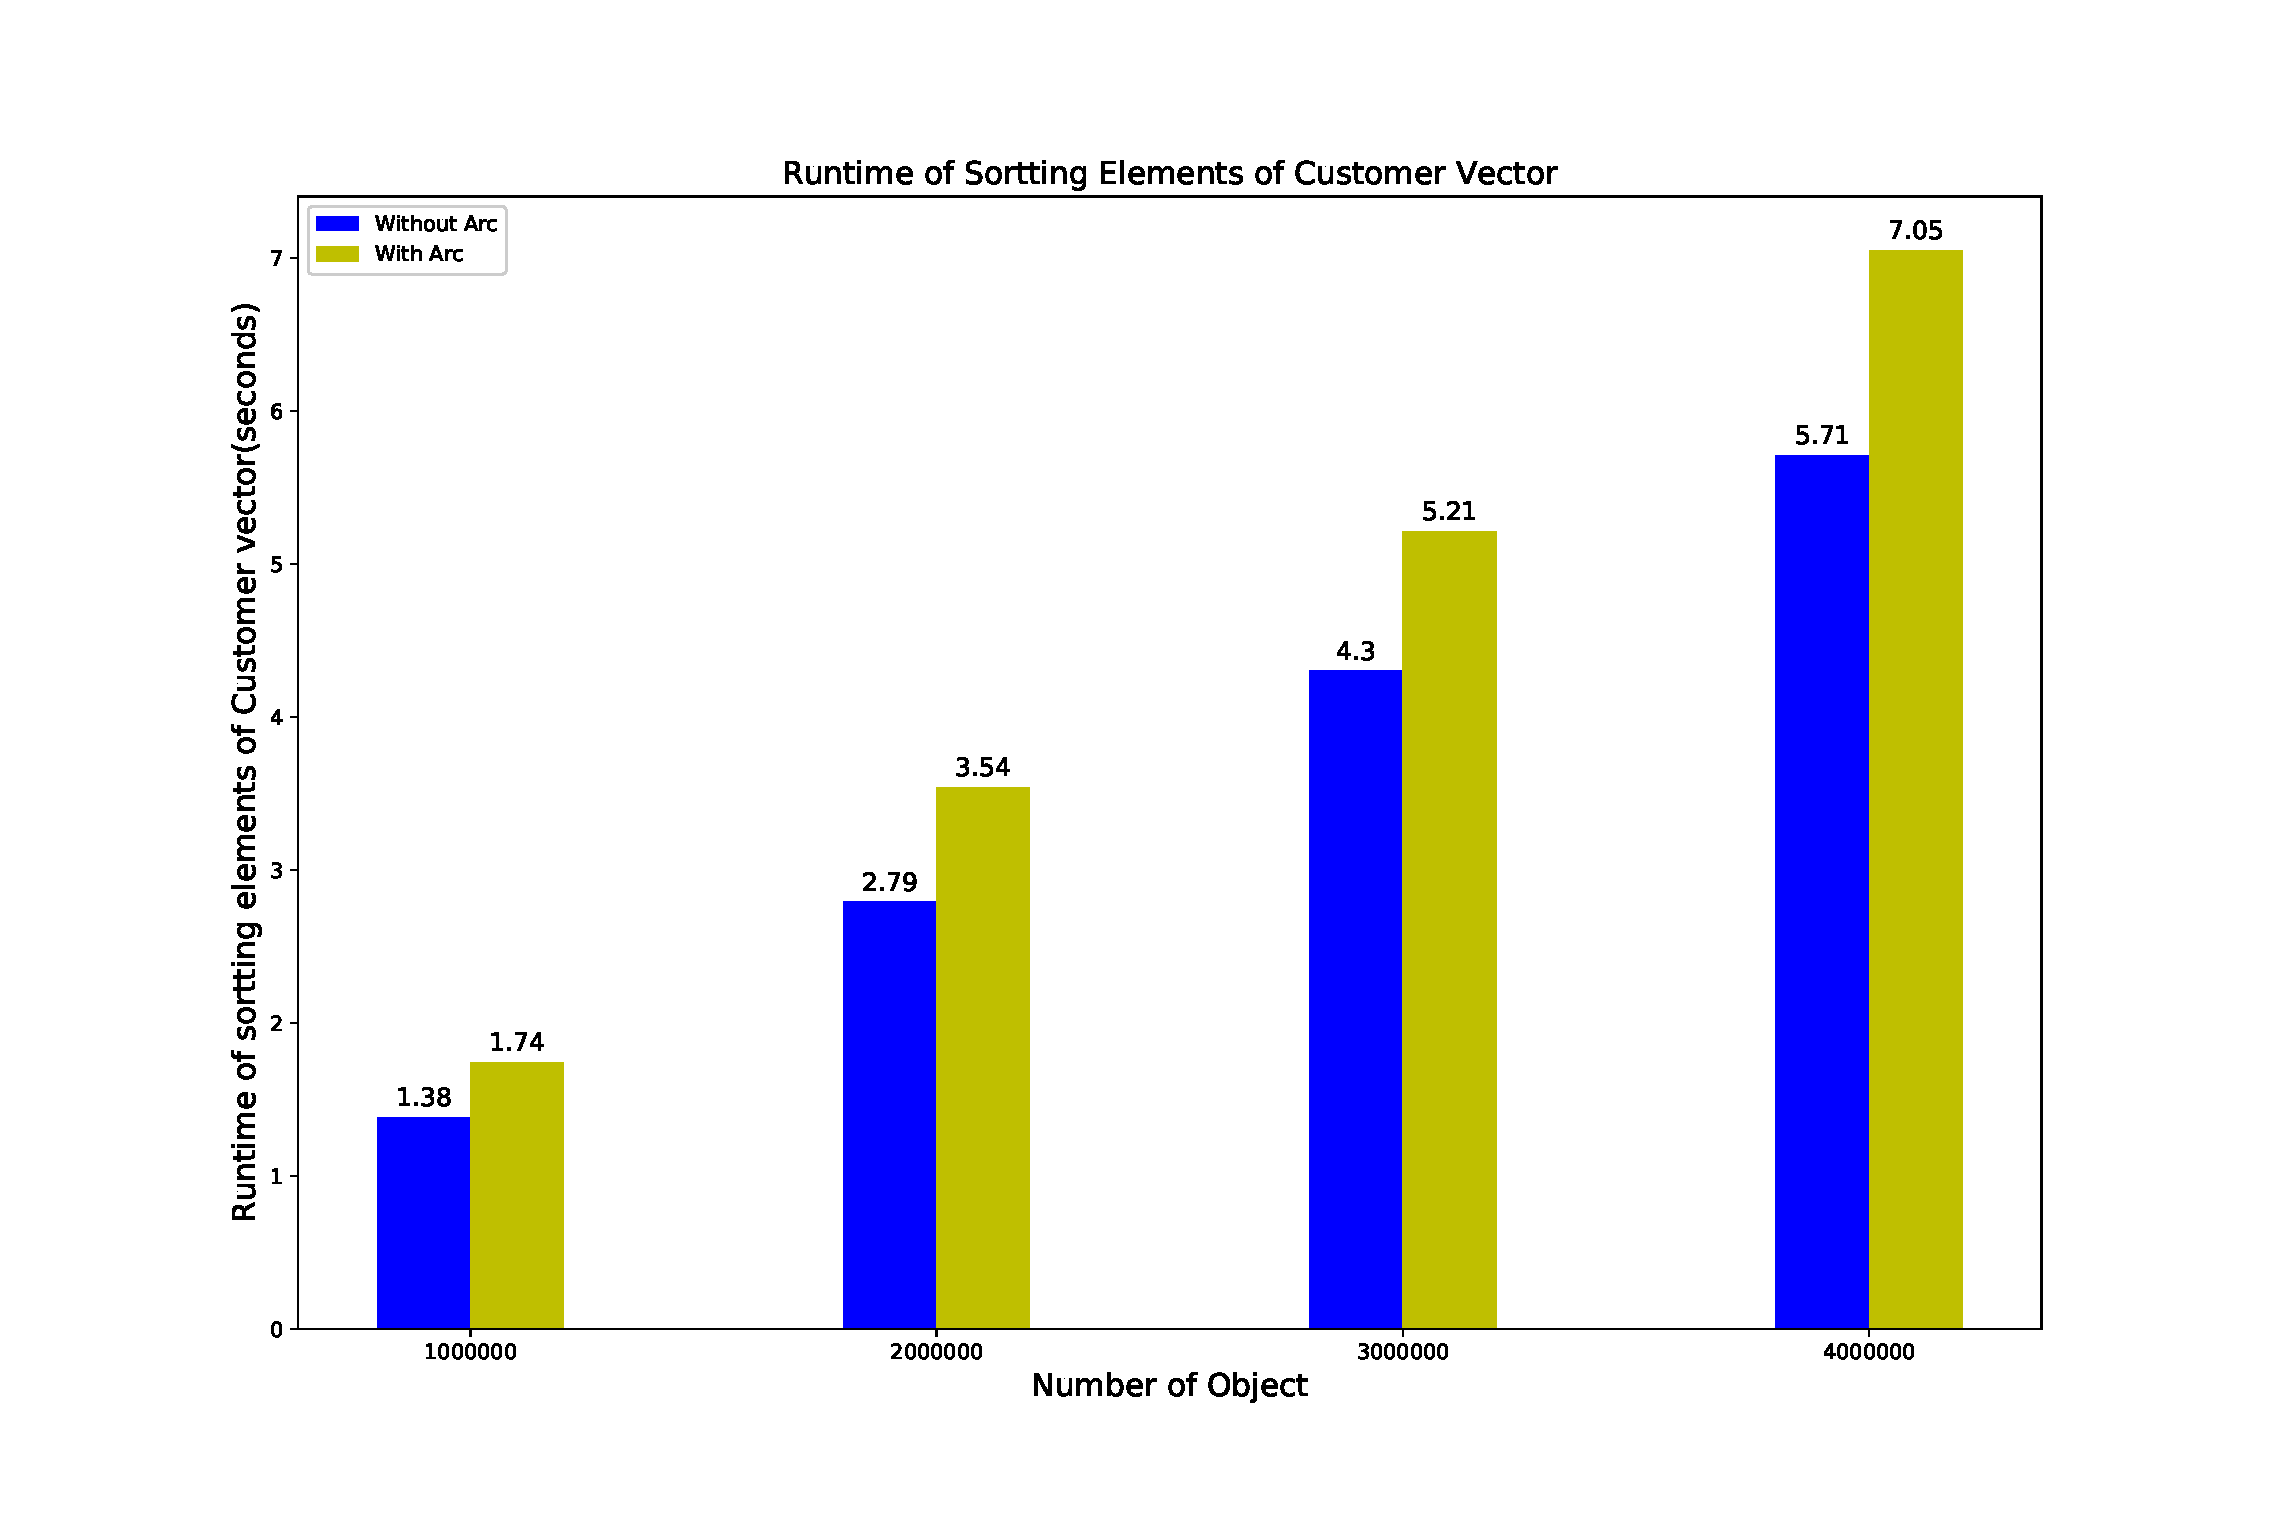
\includegraphics[width=15cm]{rust_merge_sort.eps}
    \caption{Runtime of Sortting Elements of Customer Vector}
    \label{fig:Sampling}
\end{figure}



The other is LinkedList implementation other than vector.
The linkedlist implementation is different from another two. This algorithm is inplace sorting so that it does not de/allocate memory during execution. 
The comparison among vector and linkedlist implementations can show trade-off between contiguous memory access and inplace non memory de/allocation. 
Experiment with Java linkedlist implementation can be interesting, because Java GC is severe problem when number of object is large. 
\clearpage

\section{Experiment for Tree-aggregation}
\label{sec:history}
\subsection{Description}
Tree-aggregate is a communication patten heavily used for Machine Learning algorithm in Spark (MLlib). 
In the traditional aggregation function in Spark, results of aggregation in all executor clusters are sent to the driver. 
That is why this operation suffers from the CPU cost in merging partial results and the network bandwidth limit.
Tree-aggregate is a communication pattern which overcomes these problems by breaking aggregate operation in multi-level represented like tree structure.

In our experiment, tree-aggregation algorithms are examined in multi-threading. This experiment is to evaluate the impact of having Arc (Atomic Reference Counting) as elements of vector. 
In Big Data mining tool, such as Spark, it generates intermediate objects from original source vector. In tree-aggregation, aggregated HashMap like data structure is created in each step or node. 
Acquisition of elements in source vector is required to perform this aggregation. There are several ways.

One way is deep-copy elements of vector. This solution allocated newly created objects by deep-copy. 
Aggregation is performed on copied objects, stores them in the data structure and sends it to next node. 
Deep-copy generates duplicates of objects in vector and aggregated data structure. 
This can lead to memory intensive moment when we need memory space for the duplicated objects in addition.

The other way is to get reference to the elements. Since an original source vector is deallocated after a local aggregation,
Simple reference to elements does not live long enough and allow the aggregation result to be sent to next node. 
Instead of simple borrowing, we need owner in the aggregation result. Reference Counting (Rc) in Rust is a way to have multiple owners to a value. 
Since our experiment is implemented in multithreading, Atomic Reference Counting (Arc) is used instead of Rc. With Arc, multiple ownership pointer can be 
possessed by different variables across multiple threads. Therefore a value is not deallocated until all of owners to it are dropped. 
This does not require extra memory allocation, because only acquisition of new ownership to value is needed. 
However, deletion of Arc type checks whether the value is still owned by other variables. 
This checking may be a overhead in algorithms where generate a lot of intermediate data structures, because deletion of the data structures occurs in frequent.

Two algorithms are implemented using the above two different methods and evaluated their runtime performance. 
The both algorithms perform tree-aggregation where runs seven nodes. 
Each node load Customer vector from disk and aggregate it by Customer last name. Once a node finishes aggregation, it sends result to parent node. 
After parent nodes receive aggregation results from all of its children nodes, it joins all aggregation results including its and sends next parent. 
One algorithm performs aggregation by deep-copying elements from source vector loaded from disk. In the other algorithm, each element of source vector 
is wrapped in Arc, and its reference is acquired while aggregation. 


\subsection{Result}

Figure shows runtime performance of two tree-aggregate algorithms. The runtime of algorithm with deep-copy is slower than algorithm with Arc for every vector size. 
This is result of overhead of deep-copy is larger than deletion of Arc. 

\begin{figure}[htb]
    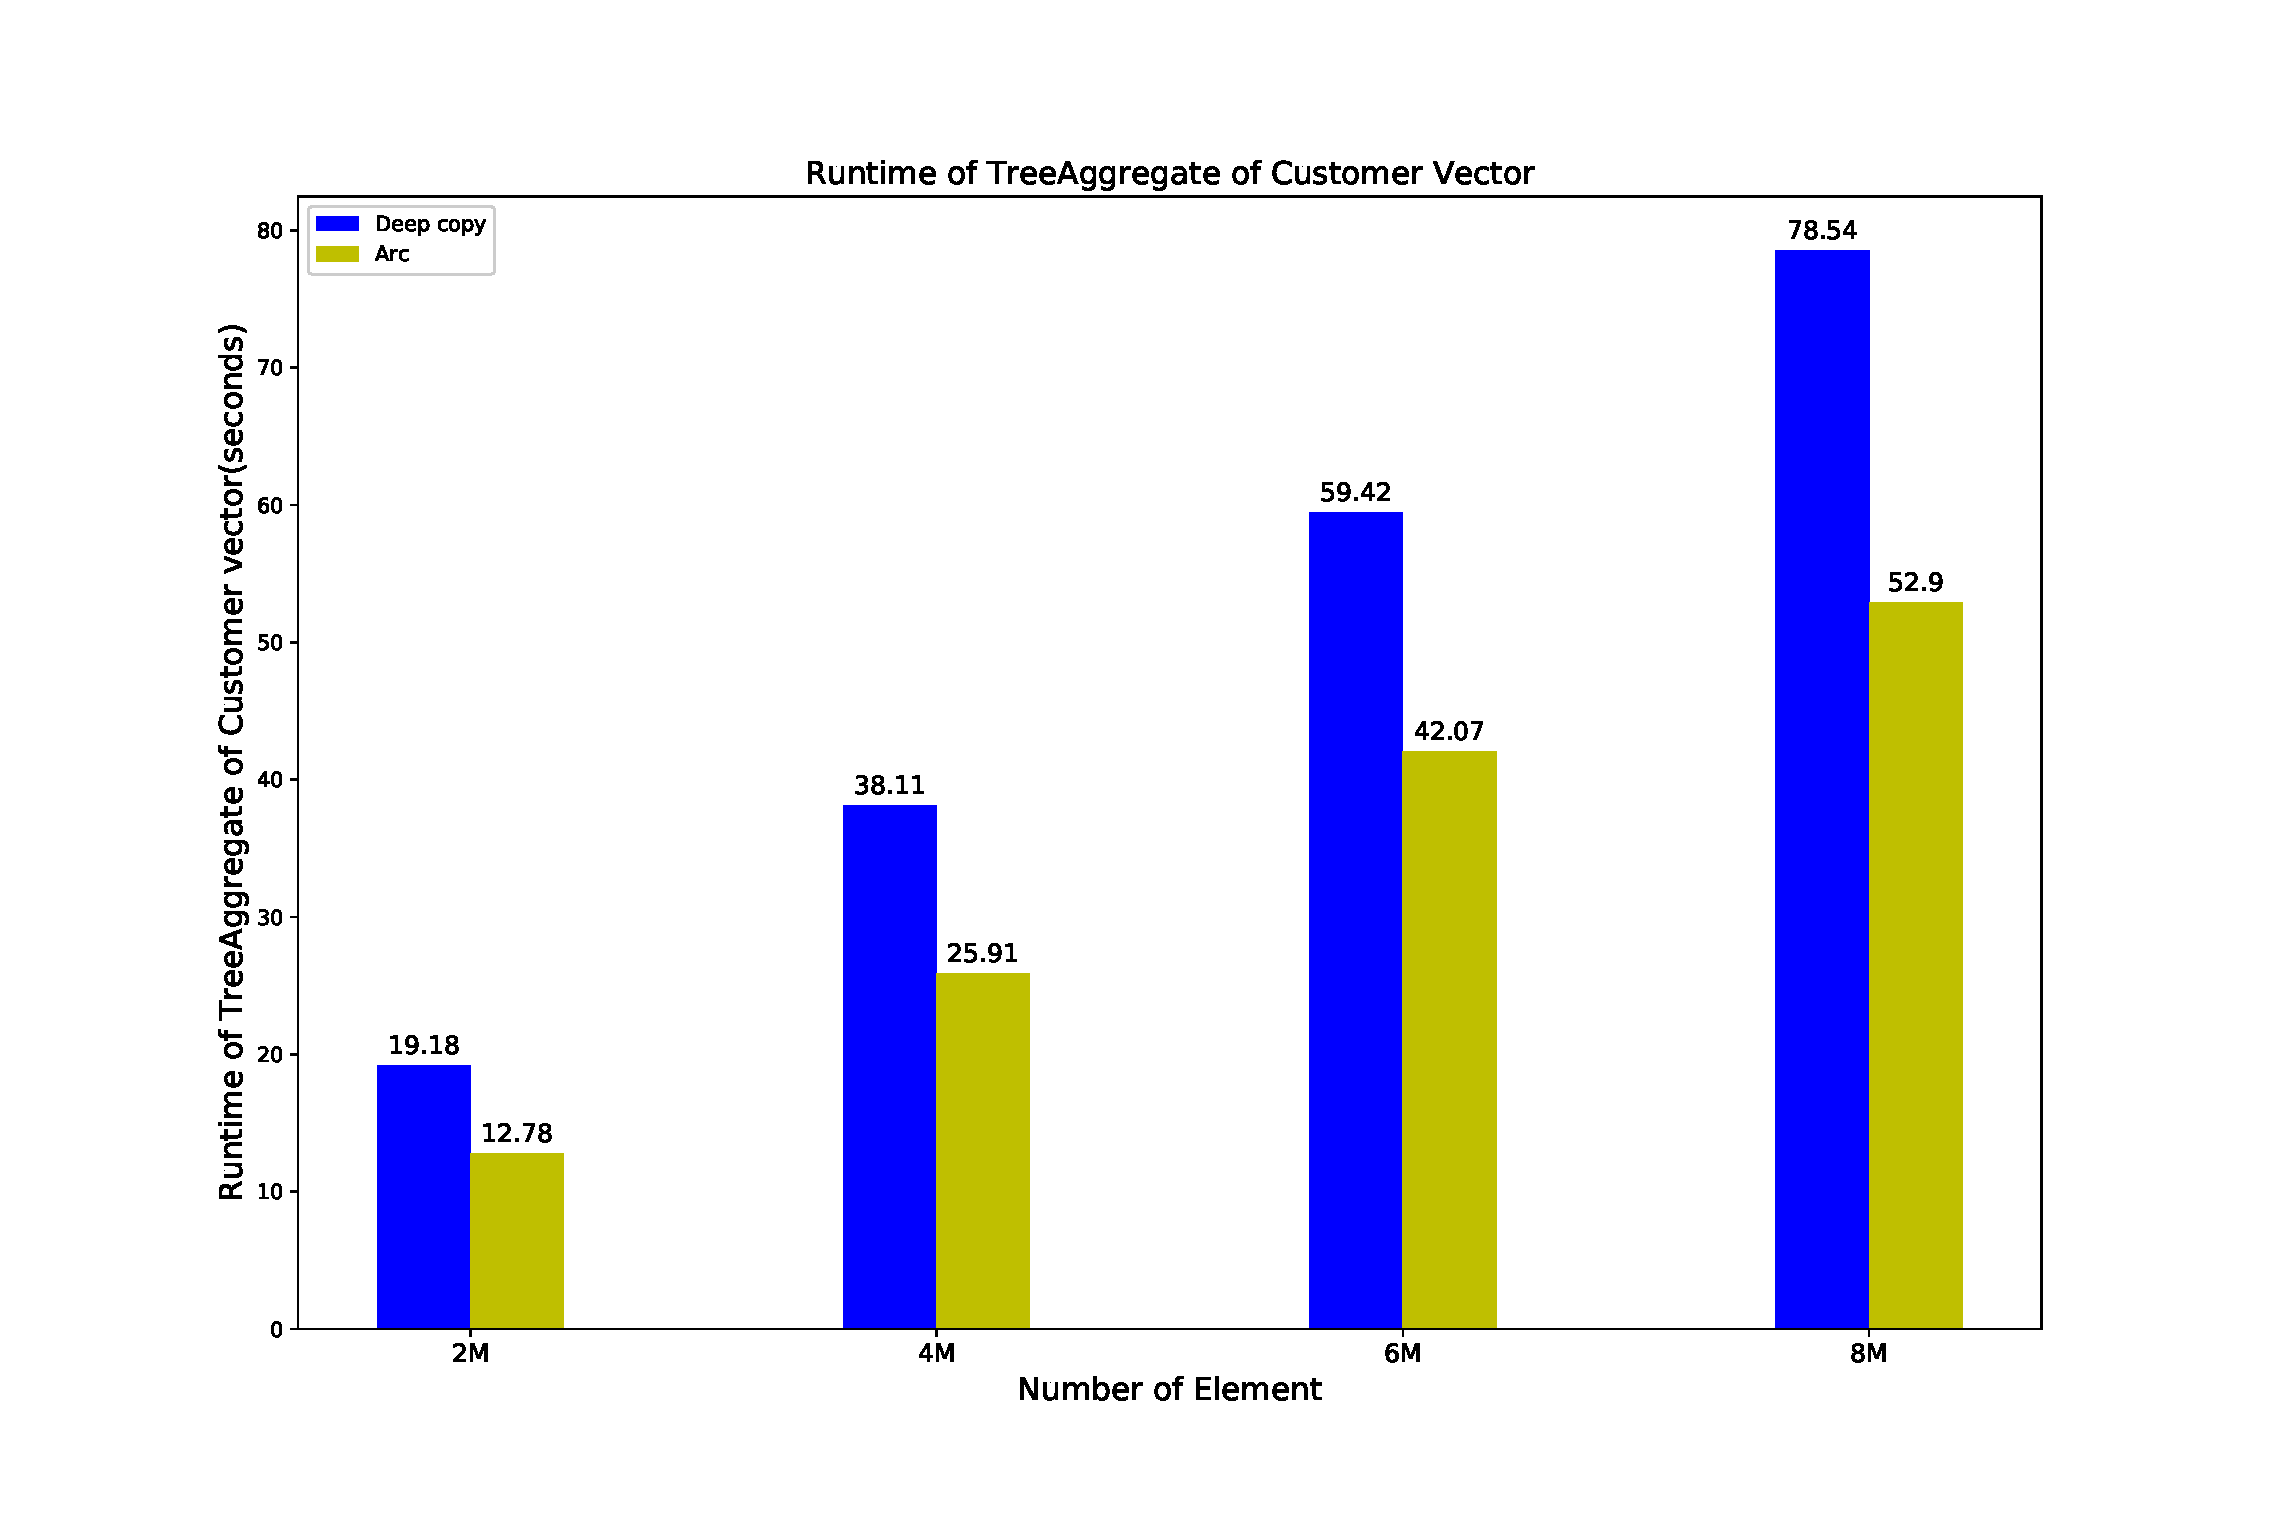
\includegraphics[width=15cm]{rust_tree_aggregate.eps}
    \caption{Runtime of Tree-aggregate algorithm}
    \label{fig:Sampling}
\end{figure}

\subsection{Discussion}
As we explained, Arc has overhead to be deleted because it has to check if the value is still referred. 
Even though the deletion of Arc is slow, deep copy of complex objects has more impact in deterioration of runtime performance. 
In the algorithm with deep copy, the elements of each partition in each node are deep-copied once during aggregation. 

If total number of elements are 1000000, the all of 1000000 elements are deep-copied once during execution. On the other hand, acquisition and deletion of Arc occurs several time for each element object.
First, acquisition of Arc of all elements in loaded vector happens during aggregation in each node and the loaded vector is deleted after the aggregation. 
Second, deletion of all elements in aggregated structures from children nodes and the node is occurs after joining these aggregated structures to single one. 

The result shows a deep-copy of Customer vector is computationally much more expensive than acquisition and deletion of Arc. 
This result suggests that having element objects in Arc is efficient than deep-copying element from original source vector in tree-aggregation algorithm 
where generates intermediate data structure. 
\clearpage


\cleardoublepage

% -------------------------------------
% CHAPTER 3: CONCLUSION
% -------------------------------------
\chapter{Conclusions}
\label{chapter:Conclusions}
\thispagestyle{myheadings}

% set this to the location of the figures for this chapter. it may
% also want to be ../Figures/3_Body/ or something. make sure that
% it has a trailing directory separator (i.e., '/')!
\graphicspath{{3_Conclusion/Figures/}}

% Quick recap of what we did 
% - The purpose of this research
% - Experiment that we conducted
In this thesis, we have presented a number of experiments to assess better implementation of algorithms 
when one develops Big Data analysis tools with Rust programming. 
Those experiments examine how different variable types, Reference Count (Rc), and different memory management strategies in Rust affect performance of algorithms.

% What we find 
% - The result of our experiments
The results show useful benchmark when one implements Big Data analysis tools.
The different variable types in Rust have similar access time to the memory address of their value. 
Therefore, we do not need to consider such access overheads. 
The drop on Rc or Arc is more expensive than ordinal variables, 
because these shared variables need to check count of reference to its actual value. 
The atomic operation used by Arc may be a cause of overhead in multithread programming in Rust. 

% What is the most significant
% - Use of Reference is depending on Complex object type
% - When we have complex object, we should use Reference count
% - Frequency of memory de/allocation has impact
One of the most notable discussion is selection of whether developers should use sharing (Rc or Arc) or deep-copy. 
In algorithms used to process Big Data, the same elements are used over and over agin. 
In Experiment 4 and 5, we implement the algorithms in different strategies and assess which implementations performs better in runtime.
The result is that the algorithms sharing elements using Arc is more efficient strategy when the shared elements are very complex objects. 
On the other hand, when the elements have light complexity, such as String, the algorithms deep-copying the elements is more faster.
Therefore, the decision of which strategy to use is dependent on how complex element objects are.

% Conclusion acquired from that
% - the design of algorithm is depend on implemetation of complex objects
% - Rust ownership memory management seem to work well
% - We can manually de/allocate memory and compiler can still ensure memory safety.
The other important discussion is how Rust ownership memory management can impact performance of algorithm.
Even though the main concept of ownership is safety of memory, programming patterns using this ownership may determine the frequency and timing of de/allocation. 
Experiment 5 shows the ownership memory management works well; the frequency and timing of de/allocation is fairly reasonable for algorithms to result good runtime performance and memory usage. 
However, when the situation is memory intensive and needs more fast runtime performance, developers need to perform more careful memory managements,such as manually specifying when to deallocate memory.
Rust can check memory-safety of these manual operation at compile time, so such optimizations can be done fairly easy.

% How our conclusion can be applied in real world 
% - Decide data structure implementation that used in Big Data Systems then
% conduct experiment that fits for the best runtime performance.
As we can see in the results of experiment, different memory strategy varies the performance of algorithms in Rust programming.
Which memory management strategy to take depends on what objects to deal with. 
Therefore, development of Big Data analysis tools in Rust programming should be started with objects implementation used in the systems.
Next, one can select suitable memory management strategies. 
Finally, algorithms can be optimized with more dedicated strategies to application setting, such as capacity of memory.
\cleardoublepage

%\appendix
\begin{appendices}
\graphicspath{{Appendix/Figures/}}

% \chapter{Operating Systems}
% \label{appendix}
% \thispagestyle{myheadings}
% \subsection{Memory and Process in Operating Systems}
\label{sec:os_mem_process}
A process is a subsection of computation job. A process can work on a CPU core. We can divide process as well.
Basically, each process does not share their memory. However, for multiprocessing, we could avoid this restriction.
Processes can be represented as tree structure, because a process may create other child processes.
Process has 4 states, new, running, waiting, and ready. 
Process is represented in process control block (PCB) with state type, process ID, registers, and so on.
The scheduling for process assigning to CPU core is implemented in queues containing PCB. There are two main queues in this scheduler: 
ready queue and wait queue. The head of process in ready queue is selected for execution and once the process requested I/O request or 
production of child process, the running process will be stored n wait queue. Once the request that the process waiting for end, 
the waiting process will be pushed tail of ready queue. 

Processes executing concurrently in the operating system may be either independent processes or cooperating processes executing in the system.
A process is independent if it does not share data with any other processes. A process cooperating if it can affect or be affected by the 
other processed executing in the system. In cooperating process, there are two kinds, shared memory and message passing. 
In shared memory, it removes restriction of not interfering memory region. Message passing can be useful for distribution systems as well.

For a pair of processes to communicate through message, a socket is needed to be established. 
A socket is identified by an IP address concatenated with a port number. When two process communicate, each process will have socket. 
If another process of the same machine wants to communicate, we need new socket to be established. The protocol used in the socket connection
can be TPC and UDP.

\subsection{Multi-threading and Parallelism}
\label{sec:os_thread}
A thread is a basic unit of CPU utilization, so that a process can have multiple thread. Threads share mainly code and data. 
Multi-threading is increasingly popular as the multicore programming becomes in common, because we can run multiple thread on different core.
Creating thread is much cheaper than creating process and it shares resources so that we do not need additional methods to allow threads to 
communicate each other, such as sharing memory and message passing.

\subsection{Memory management in Operating System}
\label{sec:os_memmanage}
In computer storage hierarchy, the closest storage to CPU is register. It is built into each CPU core and accessible within one cycle of the CPU clock.
However, the same cannot be said of main memory, which is accessed via a transaction on the memory bus. This takes many cycles of the CPU clock.
The remedy is to add fast memory between the CPU and main memory, typically on the CPU chip for faster access. Such a cache plays a role for this.

For the layout of main memory, it must be ensured that each process has a separate memory space, including operation system. 
The base register and limit register, whose roles are lower bound of memory region and specific size of range respectively, can achieve that goal. 

Usually a program resides on a disk as binary executable file. To run, the program must be brought into memory and placed within the context of a process.
The process is bound to corresponding parts of the physical memory. Binding program to memory address is staging process. 
There three stages: compile time, load time execution time. The source program is compiled by compiler producing object file. 
After the compilation, the object file is linked with other object file by linker creating executable file . 
Finally, the executable file will be loaded to run execute. At this run time dynamic library link can be done.

If where the process will reside in memory at compile time, absolute code is generated. If this is unknown at the time, 
the binding will be done at load time. At this time, the compiler must generate relocatable code. Otherwise, the binding will be done at 
execution time.

A process does not interact with addresses of physical memory, instead virtual memory. The memory-management unit (MMU) takes roles to map 
logical address to physical address. OS needs to ensure that any of physical memory spaces of processes do not overlap. 
Since one process can be created and deleted and the corresponding memory space should be de/allocated, 
optimization for use of physical memory space is important; we need to allocate memory contiguously avoiding fragmentation.

There are several approaches to deal with this problems. However, we will focus on paging here, which is the most used method OS use to manage memory.
A frame and page are a unit of Separated physical and virtual memory space in fixed size (4KB or 8KB) respectively.
A process can use as many as pages and corresponding frames obtained by page table matching. This strategy does improve external fragmentation, but not for internal fragmentation.
The smaller size of page has smaller fragmentation, but mapping from page to frame has overhead and also disk I/O is more efficient when the amount of data transfered is larger.



\subsection{Demand Paging}
\label{sec:os_paging}
A process can have multiple pages. However, loading entire executable code from secondary storage to memory is not necessarily needed to 
get jobs done. A strategy used in several operating systems is loading only the portion of programs that are needed, demand page. 

In the storage, some pages currently used are in memory and the others are in secondary storage. 
The page table specifies whether pages are valid or invalid, which means are in memory or not. 
Access to a page marked invalid causes page fault and some steps to resolve the error will be required. 

The first part of process of demand paging would be that we check an internal table to check whether the reference is valid or invalid.
If the reference is valid, the process reads the content from the memory. Otherwise, we terminates the process and find the free frame in 
physical memory. Then, we schedule a secondary storage operation to read the desired page into newly allocated frame. 
When the storage complete reading the page, we modify the internal table to indicate the page is now in memory. 
Finally, we restart the instruction that was interrupted. 

However, there would be a case where the memory does not have any free frame. In this case, a victim frame that will be replaced with new coming frame should be selected. 
To perform this selection efficiently, a modify bit is tracked for each frame or page. The modify bit represents whether the page is modified since it is loaded from secondary storage. 
If the page or frame is modified, when we swap page we need to update the content in the secondary storage. However, it is not modified, we can simply delete the frame and replace with new frame.



\subsection{Copy on Page}
\label{sec:os_copypage}
When a parent process creates child process and if these process shares contents on particular page and modify it, 
only the page which has the context will be copied.


% \subsection{Threads and Concurrency}
% \label{sec:history}

\chapter{Linear Algebra Computation}
\label{appendix}
\thispagestyle{myheadings}


\subsection{BLAS LAPACK}
\label{sec:linalg_blas_lapack}

Basic Linear Algebra Subprograms (BLAS) \cite{DBLP:journals/toms/LawsonHKK79} are standard building blocks for basic vector and matrix operations. There are 3 levels of operation. The level 1 BLAS performs scalar, 
vector and vector-vector operations, the level 2 BLAS performs matrix-vector operation, and the level 3 BLAS performs matrix-matrix operation. 

LAPACK \cite{laug} is developed on BLAS and has advanced functionalities such as LU decomposition and Singular Value Decomposition (SVD). Dense and banded matrices are handled, but not general 
sparse matrices. The initial motivation of development of LAPACK was to make the widely used EISPACK \cite{DBLP:books/sp/SmithB76} and LINPACK \cite{DBLP:journals/sigarch/Dongarra92} libraries run efficiently on shared-memory vector and parallel processors. 
LINPACK and EISPACK are inefficient because their memory access patterns disregard the multi-layered memory hierarchies of the machines, thereby spending too much time moving data. 
LAPACK addresses this problem by recognizing the algorithms to use block matrix operations, such as matrix multiplication, in the innermost loops. These block operations can be optimized for each architecture to account for the memory hierarchy, 
and so provide a portable way to achieve high efficiency on diverse modern machines. However, LAPACK requires that highly optimized block matrix operations be already implemented on each machine. 

ARPACK \cite{DBLP:books/daglib/0000896} is also a collection of linear algebra subroutines which is designed to compute a few eigenvalues and corresponding eigenvectors from large scale matrix. 
ARPACK is based upon an algorithmic variant of the Arnoldi process called the Implicitly Restarted Arnoldi Method (IRAM). 
When the matrix is symmetric it reduces to a variant of the Lanczos process called the Implicitly Restarted Lanczos Method(IRLM). The Arnoldi process only interacts with the matrix via matrix-vector multiplies. 
Therefore, this method can be applied to distributed matrix operations required in big data analysis.



\subsection{Netlib-Java}
\label{sec:linalg_netlib}
Netlib-java \cite{netlib} is a Java wrapper of BLAS, LAPACK, and ARPACK. Netlib-java choose  implementation of linear algebra depending on installation of the libraries. 
First, if we have installed machine optimized system libraries, such as Intel MKL and OpenBLAS, netlib-java will use these as the implementation to use. 
Next, it try to load netlib references which netlib-java use CBLAS and LAPCKE interface to perform BLAS and LAPACK native call. 
The last option is to use f2j which is intended to translate the BLAS and LAPACK libraries from their Fortran77 reference source code to Java class files, 
instead of calling native libraries by using Java Native Interface (JNI). 

We can use JNI to call native libraries from Java. The JNI is a native programming interface which allows Java code that runs inside a Java Virtual Machine (VM) 
to interoperate with applications and libraries written in other programming languages. 


\subsection{Matrix Computation and Optimization in Apache Spark}
\label{sec:linalg_spark_marix}

Matrix operation is a fundamental part of machine learning. Apache Spark provides implementation for distributed and local matrix operation \cite{DBLP:conf/kdd/ZadehMUYPVSSZ16}. 
To translate single-node algorithms to run on a distributed cluster, Spark addresses separating matrix operations from vector operations and run matrix operations on the cluster, 
while keeping vector operations local to the driver. 

Spark changes its behavior for matrix operations depending on the type of operations and shape of matrices. For example, Singular Value Decomposition (SVD) for a square matrix is performed in distributed cluster, 
but SVD for a tall and skinny matrix is on a driver node. This is because the matrix derived among the computation of SVD for tall and skinny matrix is usually small so that it can fit to single node.

Spark uses ARPACK to solve square SVD. ARPACK is a collection of Fortran77 designed to solve eigenvalue problems. ARPACK is based upon an algorithmic variant of the Arnoldi process called the Implicitly Restarted Arnoldi Method (IRAM). 
When the matrix A is symmetric it reduces to a variant of the Lanczos process called the Implicitly Restarted Lanczos Method (IRLM). 
ARPACK calculate matrix multiplication by performing matrix-vector multiplication. So we can distribute matrix-vector multiplies, and exploit the computational resources available in the entire cluster. 
The other method to distribute matrix operations is Spark TFOCS. Spark TFOCS supports several optimization methods.

To allow full use of hardware-specific linear algebraic operations on single node, Spark uses the BLAS (Basic Linear Algebra Systems) interface with relevant libraries for CPU and GPU acceleration. 
Native libraries can be used in Scala are ones with C BLAS interface or wrapper and called through the Java native interface implemented in Netlib-java library and wrapped by the Scala library called Breeze. 
Following is some of the implementation of BLAS.

\begin{itemize}
    \item f2jblas -  Java implementation of Fortran BLAS
    \item OpenBLAS - open source CPU-optimized C implementation of BLAS
    \item MKL - CPU-optimized C and Fortran implementation of BLAS by Intel
\end{itemize}

These have different implementation and they perform differently for the type of operation and matrices shape. 
In Sark, OpenBlas is the default method of choice. BLAS interface is made specifically for dense linear algebra. 
Then, there are few libraries that efficiently handle sparse matrix operations.

\subsection{Memory Management of each Linear Algebra Library}
\label{sec:linalg_memmanage}

The pure Java linear algebra library, such as La4j, EJML, and Apache Common Math, 
use normal GC performed by JVM to manage memory. This is because the implementation of these libraries are in purely Java.

Netlib-java, Jblas or other simple Java wrapper of BLAS, LAPACK, and ARPACK with Java Native Interface (JNI) use normal GC as well. 
This is because the native code deals with Java array by obtaining a reference to it. After the operation, 
the native method releases the reference to the Java array with or without returning new Java array or Java primitive type object. 

ND4J \cite{nd4j} has two types of  its own memory management methods, GC to pointer of off-heap NDArray, and MemoryWorkspaces. 
ND4J used off-heap memory to store NDArrats, to provide better performance while working with NDArrays from vative code such as BLAS and CUDA libraries. 
Off-heap means that the memory is allocated outside of the Java heap so that it is not managed by the JVM’s GC. NDArray itself is not tracked by JVM, 
but its pointer is. The Java heap stores pointer to NDArray on off-heap. When a pointer is dereferenced, this pointer can be a target of JVM’s GC and when it is collected, 
the corresponding NDArray will be deallocated. When using MemoryWorkspaces, NDArray lives only within specific workspace scope. 
When NDArray leaves the workspace scope, the memory is deallocated unless explicitly calling method to copy the NDArray out of the scope.


\end{appendices}
%==========================================================================%
% Bibliography
\newpage
\singlespace
\bibliographystyle{apalike}

% each subdirectory can have its own BiBTeX file
\bibliography{thesis}
\cleardoublepage

%==========================================================================%
% Curriculum Vitae
\addcontentsline{toc}{chapter}{Curriculum Vitae}

\thispagestyle{empty}

\begin{center}
{\LARGE {\bf CURRICULUM VITAE}}\\
\vspace{0.5in}
{\large {\bf Joe Graduate}}
\end{center}

Basically, this needs to be worked out by each individual, however the same format, margins, typeface, and type size must be used as in the rest of the dissertation. 
 

%==========================================================================%
\end{document}
